%%%%%%%%%%%%%%%%%%%%%%%%%%%%%%%%%%%%%%%%%%%%%%%%%%%%%%%%
%%%
%%%  LaTeX template for InTech Journal article
%%%
%%%  IMPORTANT NOTICE:
%%%  Due to the double blind peer review process, 
%%%  make sure to omit the author information from the manuscript. 
%%%  You will be asked to enter these information separately during author
%%%  registration in InTech MTS system.
%%%
%%%  Submitted content will be processed through XML workflow, so 
%%%  final PDF will not be generated from this LaTeX template.	
%%%
%%%%%%%%%%%%%%%%%%%%%%%%%%%%%%%%%%%%%%%%%%%%%%%%%%%%%%%%

\documentclass{intech-journal}
\usepackage[utf8]{inputenc}
\setlength{\belowcaptionskip}{-4pt}
\usepackage{enumitem}
%%%%%%%%%%%%%%%%%%%%%%%%%%%%%%%%%%%%%%%%%%%%%%%%%%%%%%%%
%%% 
%%%  Note that amsfonts,amstext,amssymb,amsmath,amsthm,amscd
%%%  bm,paralist,color,graphicx,array and subfigure packages
%%%  are all part of intech-journal.cls
%%%  Please avoid using additional packages.
%%%
%%%%%%%%%%%%%%%%%%%%%%%%%%%%%%%%%%%%%%%%%%%%%%%%%%%%%%%%




\articletitle{R2T2 : Robotics to Integrate Educational Efforts in South Africa and Europe } % To break lines in long titles use \\


\begin{document}
\maketitle

\articleabstract{
This paper presents the first cross-continental collaborative robotic event based around education.
It was entitled \emph{R2T2} and it involved more than 100 children from Europe and Africa. 
Based on remote programming, video streaming feedback, and a scenario of collaborative space rescue, R2T2 focused on pedagogical elements that are fundamentally different than those characterizing classic robotic competitions. 
The value of these educational actions is shown through the results of a survey conducted among the participants; the working methodologies by the African students were significantly enhanced and there was a broad inclusion in general, despite the fact that some gender issues lingered.
This paper's contribution is to demonstrate an approach to implementing a north-south collaboration to get school students excited about robotics and the problem-solving skills required in engineering. 
%limited to 190words
}
\keywords{Rescue, Educational Robotics, Thymio robot, Space Robotics, Programming}

\section{Introduction}
The South African government is working to improve Science, Technology, Engineering, and Mathematics (STEM) interests within schools in order to enthuse students about careers in these areas, which suffer from a lack of specialists in this country. 
As mechatronics engineering and robotics are mainly a combination of mechanical, electronic, and computer engineering disciplines, this initiative will enhance the skills required to work in these areas. 
Robots have been proven to be a great tool for the teaching of abstract concepts, from mathematics to mechatronics~\cite{benitti2012exploring, Karim2015}.



African students' learning activities are influenced by various factors, such as toilet facilities, building infrastructure, computer equipment facilities and laboratories,  libraries, and teaching support~\cite{sedibe2011inequality}. 
In addition, poverty, poor housing, inadequate skills development, lack of energy sources, inadequate drinking water and sanitation, poor communications, poor education and training, lack of transport, lack of sporting, and recreational activities and cultural deprivations are just a few of the factors that have led to disadvantages for these students; Apartheid is frequently blamed for this situation~\cite{mokoena2009improving}. 
Even 21 years after Apartheid finished, conditions have not necessarily improved; in fact, the reverse appears often to be true.
\\
\hspace{1cm}Many of the abovementioned problems are intrinsically related to a lack of engineering skills. 
Developing these skills, especially those relating to with mechanical, electronic, and computer engineering, could improve the living conditions of many. 
A person who has the incentive to learn in order to solve their problems can accomplish great things.
This has been seen in Malawi, for example, where people with no education were able to learn the skills necessary to build windmills as a means to generate electricity and pump water~\cite{Sheerin2009}.


With the aim of promoting robotics, South Africa has hosted educational events such as the First Lego League South Africa~\cite{FLLSA}, First Tech Challenge South Africa~\cite{FTCA}, and the World Robotics Olympiad~\cite{WRO}, and has participated in the RoboCup Junior contest~\cite{ferrein2011robocup}. 
These events have been shown to be very beneficial for students in terms of motivation for learning \cite{deci1985intrinsic}. 
They frequently encourage both autonomy and collaboration within each team of participants.
Unfortunately, such activities and events are often restricted to the upper-class schools, which have computer facilities, an internet connection, and teachers who are enthusiastic about educating their students with the help of resources that are superior to those available in the normal syllabus. 
For example, some pupils are able to attend robotics workshops at the Cape Town Science Center as an extra mural activity; however, there is a fee required to attend these sessions~\cite{Capets}.

Robotics events to promote STEM are also organized in Europe, raising similar issues in a different context.
European robotics competitions tend only to attract participants who are already interested in STEM topics, and have very little impact on wider society.~\cite{riedo2013upgrade}.
In addition, very few women participate in these events, which widens the gender gap in technology education~\cite{riedo2013upgrade}.
To some extent, the elitist aspect of these competitions is similar to what is seen in South Africa, even if it is expressed differently.
Another common characteristic of existing events is that they are all based on competitive activities. 
Surveys suggest that collaborative activities could attract more newcomers to the field~\cite{riedo2013upgrade}.

To summarize, both in South Africa and Europe, it is hard to bring robotics into schools for different reasons. 
In South Africa, the economic factor plays a more central role, but the comfort of European teachers with the status quo is also a barrier to changes.
In both regions, it would be beneficial to instigate activities that generate a broader interest, better motivate the teachers, can reach a wider cross-section of people, and are economically affordable.


When addressing these problems, the first issue is choosing a robot.
Many different robotics kits are available for STEM education. 
The Thymio II robot has been demonstrated to be an appropriate robotic platform for the furthering of STEM in Africa~\cite{Gyebi2015}, as it is an open source platform with a sensory system that includes a microphone, IR proximity sensors, a temperature sensor, an odometer, and accelerometers, combined with the use of the open source programming language Aseba~\cite{magnenat2010aseba}. 
The Thymio robot has been widely used in European schools~\cite{roy2015inirobot}, and used as a tool for teaching many topics, from physics~\cite{Mubin2013} to computer science~\cite{magnenat2014}. 
Although the Thymio robot is one of the more expensive educational robots to be used in Africa~\cite{Gyebi2015}, it is far cheaper than the Lego Mindstorm EV3 robots, and is one of the best robots in terms of processing, sensors, deployment, development, and maintenance.


This paper presents an education activity entitled R2T2 (Remote Rescue using Thymio2), which addresses the abovementioned issues by taking advantage of the opportunities afforded by the Thymio robot. 
In contrast to existing events, R2T2 is centered around a collaborative task that is based on a rescue operation wherein several groups must cooperate.
To enhance the attractiveness of the program, the rescue scenario is set on a Mars station. 
Accordingly, the participants must access the physical station model remotely.
This has several advantages. 
First, the set-up is cost-effective, as the expense of the installation is centralized but nobody needs to travel.
In addition, this arrangement allows to bring together people from different cultures and technical backgrounds who live in far-flung places. 
Specifically, it allows European and African children to collaborate, which allows for very interesting interactions whereby children can emulate and help each other.
This scenario also enables the introduction and justification of a key aspect of interaction with robots: a delay between commands issued to the robot and video feedback. 
This delay is necessary to ensure video streaming, but also realistically reflects an operation on Mars.
From an educational perspective, this delay defines the way participants can interact with their robots, excluding the possibility of remotely controlling the robots and forcing the participants to program them.
Finally, our R2T2 rescue scenario requires the coordination of 16 teams controlling 16 robots placed in the Mars station, and therefore allows the inclusion of aspects that transcend robot programming: coordination within the team and with other teams, communication, planning, validation of distant results, and so on.
This broad spectrum of activities enables the inclusion of teachers from various disciplines and participants with diverse interests.

The first R2T2 event took place in November 2015, bringing together more than 100 participants from Europe and Africa. 
A survey allowed for the identification of the interest and value of this event, as well as the specificity of the European and African participants.

The next section will introduce the Thymio robot and the R2T2 event. 
We will then introduce the survey conducted among the participants, followed by an analysis of the results. 
This will be followed by a discussion and conclusions.


\section{The R2T2 event}

This section addresses the robotic infrastructure used in the event and the concept behind R2T2.

\subsection{The Thymio robot}

The Thymio II robot, which will be referred to simply as Thymio in this article, is a desktop differential drive robot (see Figure~\ref{fig:thymio}).

Measuring 112 x 110 x 55 mm, its shape allows it to be placed on a table in several positions, allowing it to have diverse functions in addition than a mobile robot.
Its white color was chosen in order to achieve a look that is age- and gender-neutral \cite{riedo2013thymio}.
Despite its affordable price (around 130\$), Thymio has an interesting set of sensors, which are listed in Figure~\ref{fig:thymio}.
A very specific feature of Thymio is the high number of LEDs placed over its body, allowing a visualization of the sensors' activities and creating a high degree of interactivity with the user.
At the software level, Thymio supports the ASEBA framework\cite{magnenat2010aseba}, consisting of a virtual machine running in the robot processor and a very flexible communication infrastructure enabling the programming of the robot and the running of debugging tools over many communication channels. 
For R2T2, we use the ability to connect to the robot from a computer through a radio protocol, before using a switch to enable connection from anywhere via the Internet.

\begin{figure*}[ht]
 \centering
    \includegraphics[width=0.9\columnwidth]{figures/thymio.pdf}
  \caption{The Thymio robot and its sensors.}
  \label{fig:thymio} 
\end{figure*}

There are several programming interfaces that can generate code for the onboard ASEBA virtual machine, of which the three main ones:
\begin{enumerate}
\item A text-based environment, illustrated to the left in Figure~\ref{fig:programming}, enabling the use of a simple matlab-like scripting language.
\item A graphic environment entitled \textit{VPL} and illustrated on the right in Figure~\ref{fig:programming}, allowing programming for beginners, even non-reading children.
\item Scratch and Blockly environments that use a graphic layout to place text-based code.
\end{enumerate}

\begin{figure*}[ht]
 \centering
    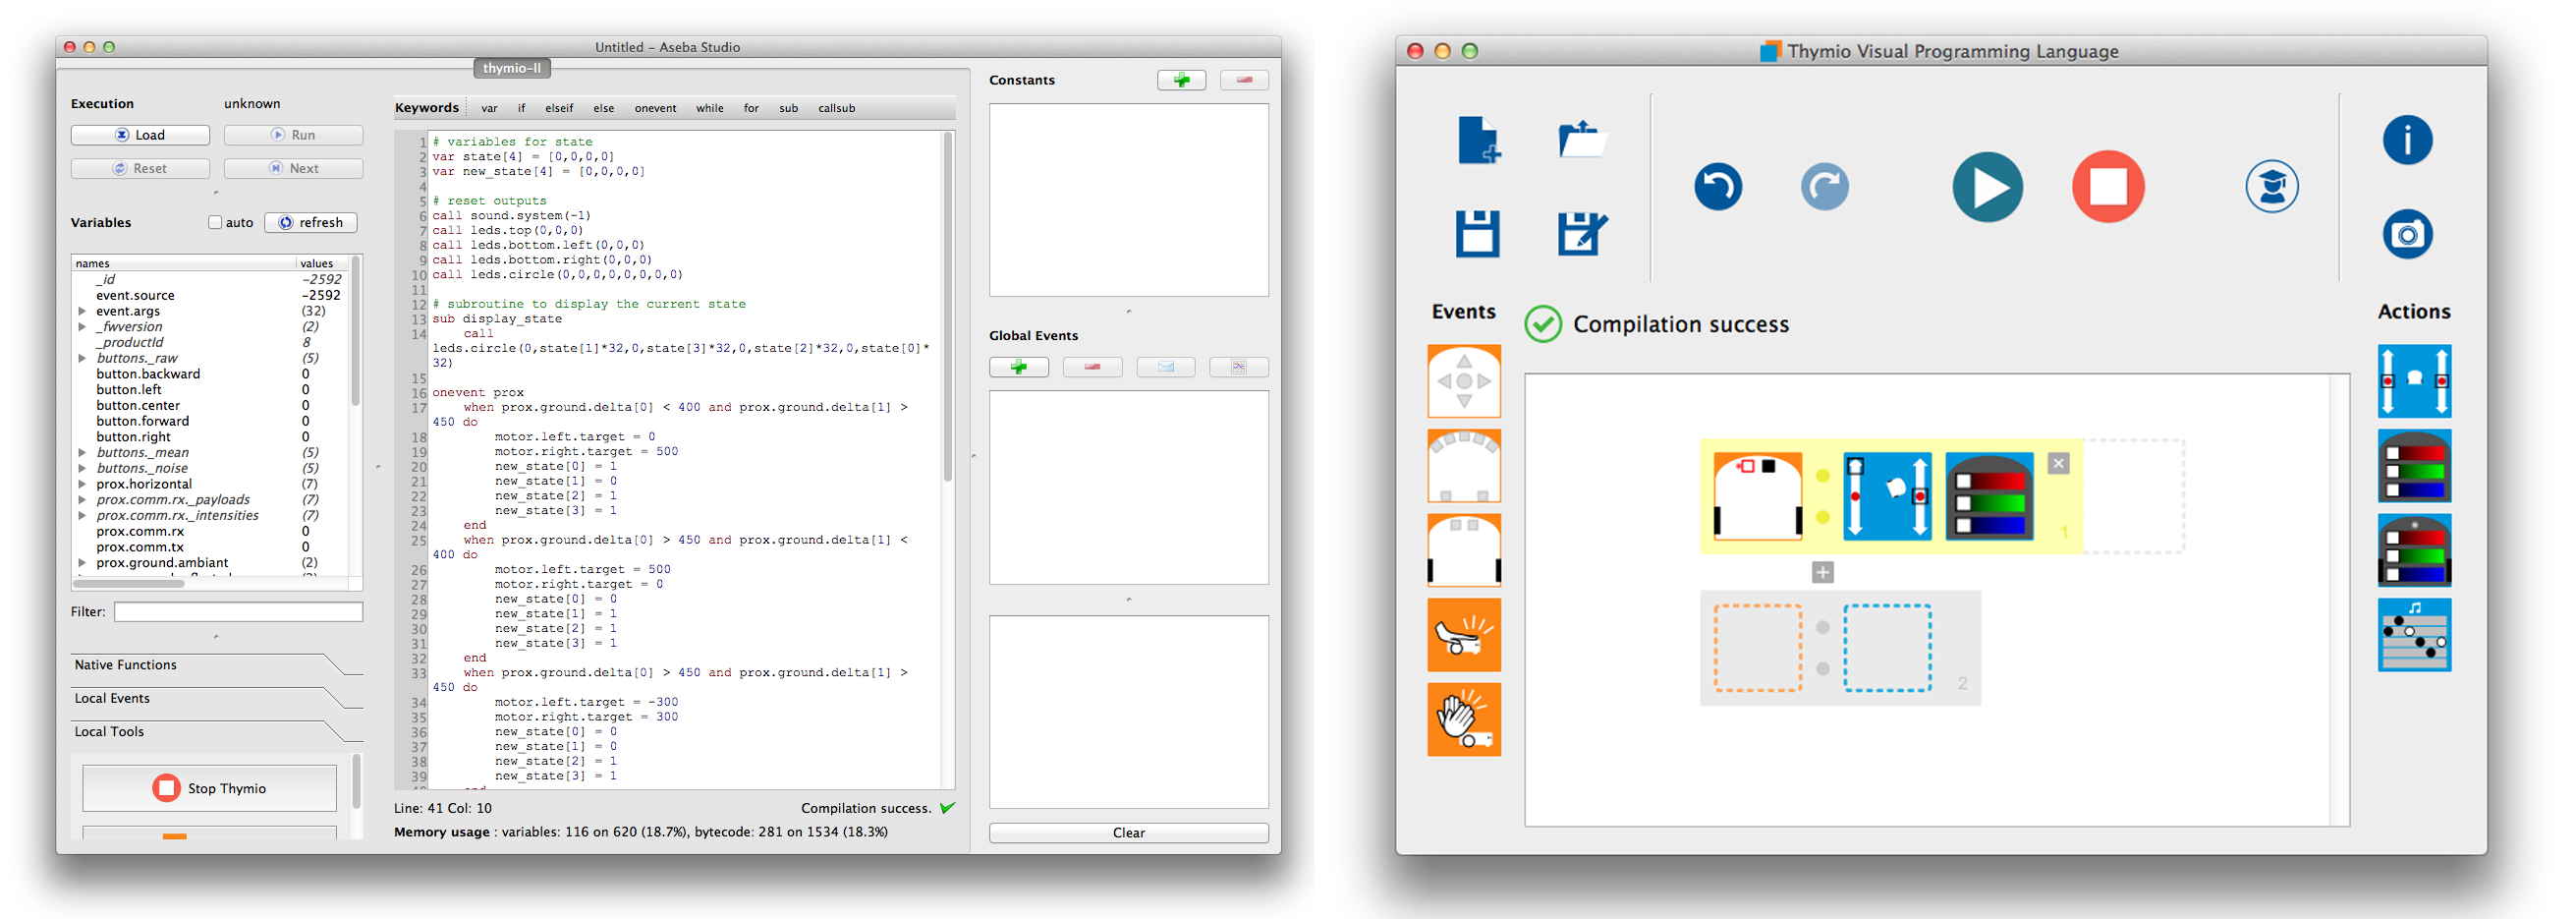
\includegraphics[width=0.9\columnwidth]{figures/studio-VPL.png}
  \caption{The two main Thymio programming interfaces: on the left, the text interface, allowing real-time visualization of variables, debugging, and so on. On the right, the graphical interface for beginners, enabling the definition of sensor-action associations that can define a behavior.}
  \label{fig:programming} 
\end{figure*}

\subsection{The R2T2 concept}

The R2T2 concept aims to bring together a large number of children from everywhere on the planet, and from Africa in particular, for a highly visible and motivational event that teaches them about STEM.
One method of keeping the budget as low as possible is to let the participants access the event and control the robots remotely, saving money on travel and the cost of the central installation.
Space exploration is one well-known application based on remote operation of mobile robots.
For children, the use of robots on Mars is very appealing as it is related to current events (the exploration of Mars) and movies (such as \textit{The Martian}).
Therefore, it was decided to create a scenario around space robotics.

Once the environment and the mode of access to the robots is set, the next question relates to the tasks to be solved.
Since existing surveys demonstrated that society at large is more likely to engage in collaborative activities than competitive ones~\cite{riedo2013upgrade}, it was decided to instigate a cooperative task instead of a traditional robot competition. 
Among the applications that are addressed at École Polytechnique Fédérale de Lausanne (EPFL) in the National Center for Competence in Research \textit{Robotics} that supports this initiative, search and rescue has a central role.
Therefore, the following R2T2 story was developed (see illustration in Figure \ref{fig:illustration}):
\begin{quotation}
``We are in 2032. A meteorite has damaged an important Martian power station and we need to assess the damage and restart the main generator. We have 16 robots on site. Each robot can be controlled by a team of engineers and space experts from Earth. Between Mars and Earth there is a delay in video transmission (between 3 minutes when Mars is closest and 21 minutes when Mars is farthest from Earth in its orbit) and direct remote control is impossible. Therefore the Earth experts need to program the robots to solve the task. We recruited 16 teams of experts from Switzerland, France, Austria, Italy, Russia and South Africa.''
\end{quotation}
16 teams were recruited: eight from Switzerland (two from Sion, two from Geneva, one from Lausanne, one from Fribourg, one from Z\"urich, and one from Founex), one from Italy (Borgonovo Val Tidone), four from France (Ayguemorte-les-graves, Floirac, Talence, and Vandoeuvre les Nancy), one from Austria (Graz), one from Russia (Moscow), and one from South Africa (Durban). 
For this first edition, it was decided to take only one team from Africa and use a network of known partners to test the concept in order to ensure a better chance of success.

\begin{figure*}[ht]
 \centering
    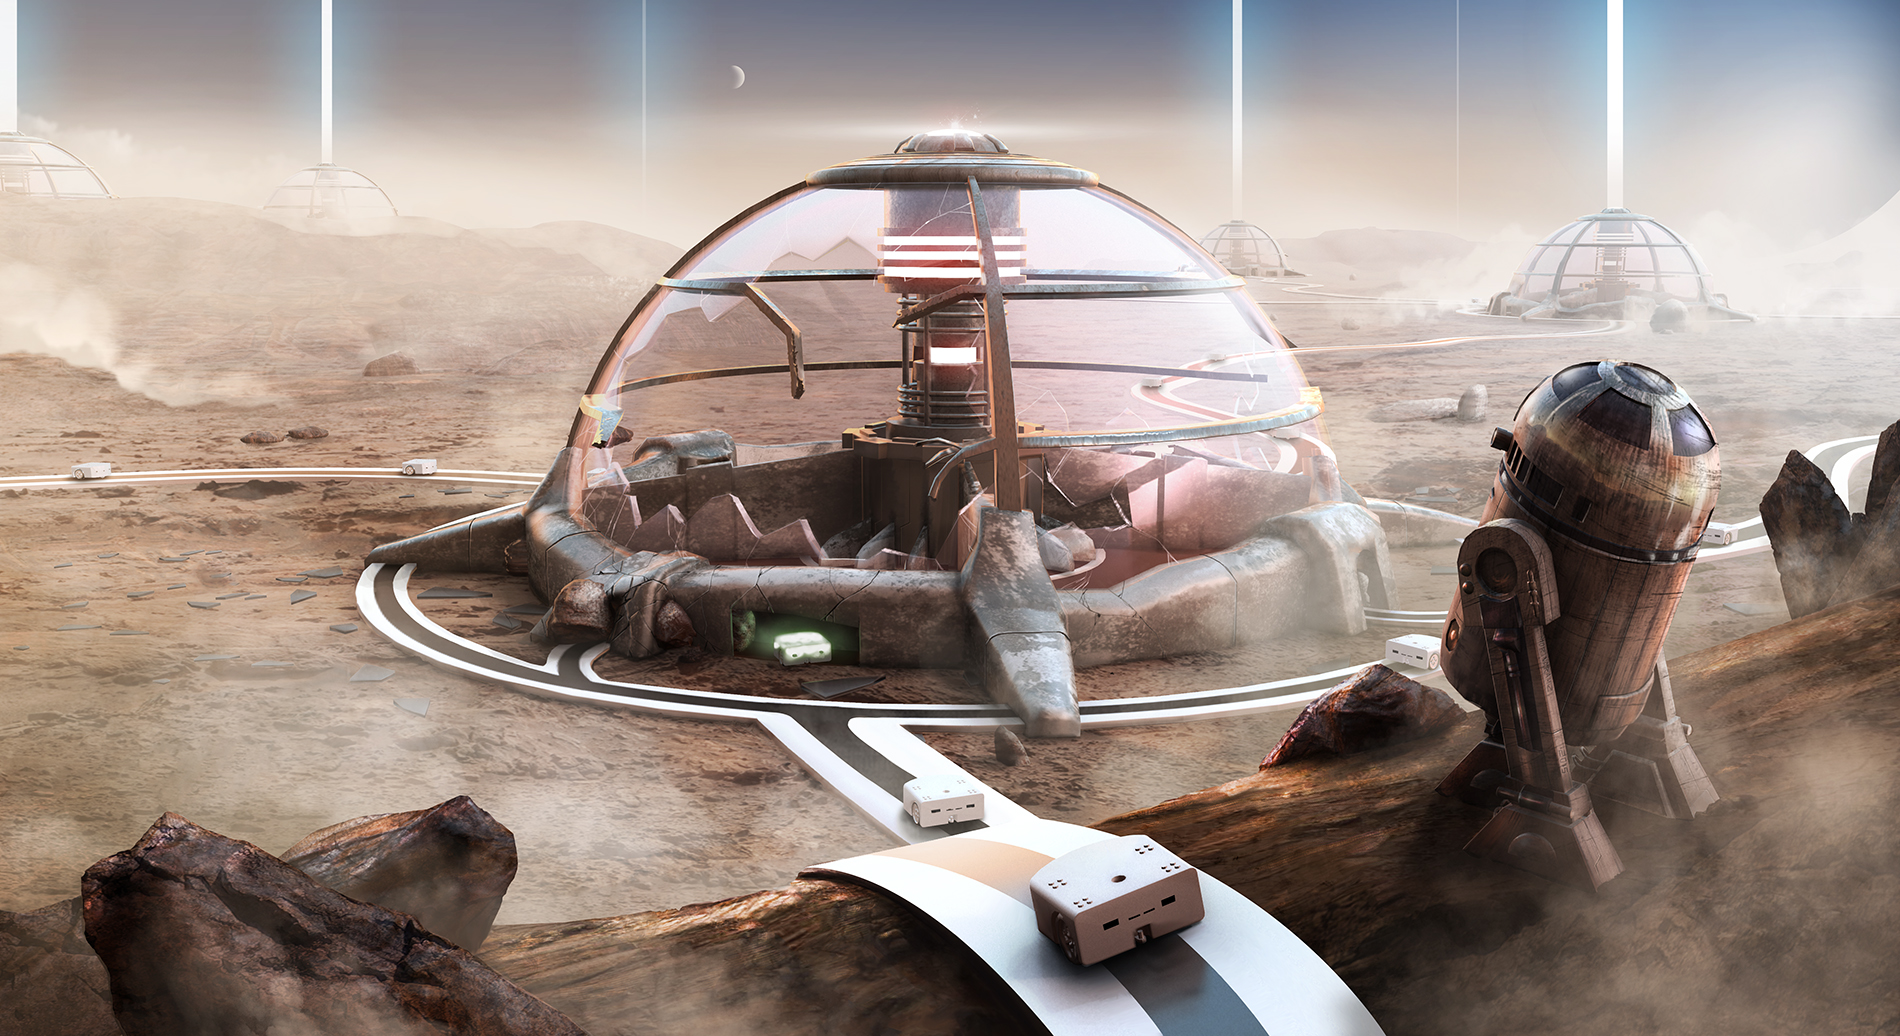
\includegraphics[width=0.65\columnwidth]{figures/r2t2_illu.jpg}
  \caption{Artistic illustration of the R2T2 space rescue scenario.}
  \label{fig:illustration} 
\end{figure*}

Each team could access and program a Thymio robot located around the Mars station model located in Lausanne. 
Video feedback was provided via live streaming on YouTube, where a chat facility was also provided to enable the exchange of messages between the teams.

The Mars station (see map in Figure \ref{fig:map} and pictures in Figure \ref{fig:setup-physical}) simulated a power plant with a central generator surrounded by four identical sectors referred to as A, B, C, and D.
Each contained a main door that was obstructed by a collapsed structure, as well as a back door, a control zone, and a generator observation zone.
Four Thymio robots were located outside each sector. 
Their rescue mission consisted of five stages:
\begin{enumerate}
\item Entering the station. This phase required one of the four robots to enter by the back door and push away the obstacle obstructing the main door. All robots could then enter the control zone.
\item Finding the control spots. In the control zone, there were four white dots on the black floor. Each robot had to place itself on one of the dots in order to activate access to the generator.
\item Looking into the generator. Once the access was activated in all four sectors, each robot had to place itself in a slot around the generator. Each slot had a small window allowing a view into the generator. By using a proximity sensor, each robot could detect when the rotor of the generator was in front of the window.
\item Evaluating the generator speed. In this stage, each robot switched on a light when it saw the generator rotor, and switched it off when the rotor could no longer be seen. This enabled an estimate of the rotational speed of the generator from the outside.
\item Restarting the generator. This final phase was simply spectacular, as the generator started spinning faster and faster, demonstrating the success of the mission.
\end{enumerate}

\begin{figure*}[ht]
 \centering
    \includegraphics[width=0.6\columnwidth]{figures/map.pdf}
  \caption{Map of the 4m x 4m Mars station model with the five phases of the rescue mission.}
  \label{fig:map} 
\end{figure*}

\begin{figure*}[ht]
 \centering
    \includegraphics[height=45mm]{figures/setup.pdf}
    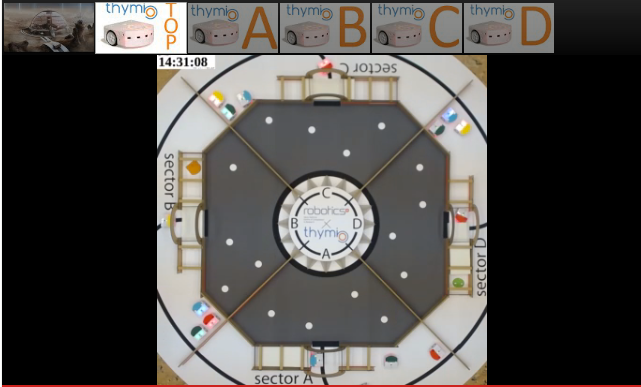
\includegraphics[height=45mm]{figures/youtube-view.png}
  \caption{Physical setup in EPFL Lausanne and view of the station on YouTube.}
  \label{fig:setup-physical} 
\end{figure*}

To provide feedback to the users, five cameras were placed around the station (see Figure \ref{fig:setup-physical} to the left), one for each sector and the fifth providing a general top view (see Figure \ref{fig:setup-physical} to the right).
In the first three stages, the participants could get a detailed view of their sector through its specific camera, as well as an overview from the top camera.
Each view had an associated chat window, allowing the exchange of messages between the people active in that area and an operator in charge of the sector, who was physically located in Lausanne near the station model (see Figure \ref{fig:setup-physical} to the left).
The need for communication between the teams obliged us to choose an official language. 
As the majority of team were French-speaking, this language was chosen.

The technical infrastructure supporting the video streaming and the control of the robots is presented in Figure \ref{fig:setup-scheme}.
Behind each camera there was a server encoding the video and streaming it to the YouTube servers. 
The whole process of encoding, transmitting to the YouTube servers, dispatching to YouTube clients and visualizing, entailed a delay of 30-60 seconds.
The same computers that were in charge of the video streaming of the four sectors were also used as bridges for the robot control. 
In fact, the control came from the participants via the Internet, and was then routed to the robots through a radio connection. 
Through this channel, each participant could both visualize the robot data and transmit motor commands or programs to be executed by the robot. 
Although the exchange of data and programs with the robots was accomplished with very slight delays, the effect of the programs or motor commands could be observed only after the delay of the video transmission. 
From a very detailed technical point of view, this does not match the behavior of remote teleoperation on Mars, but the final result for the participants is very similar.

\begin{figure*}[ht]
 \centering
    \includegraphics[width=\columnwidth]{figures/setup-schematic.pdf}
  \caption{Infrastructure of the R2T2 experiment.}
  \label{fig:setup-scheme} 
\end{figure*}

\subsection{The preparation of the teams}

Each team was very different in organization, age, and motivation.
Some teams were organized by schools, others by parents, by associations, by shops, or by universities. 
Those that were not in French-speaking regions had an additional responsibility of looking for a French-speaking person to be in charge of the communication. 
This was particularly the case for the Russian, Italian, Austrian, Swiss (Z\"urich), and South African teams. 
Most of them had a French teacher among their coaches or ensured they had a French-speaking participant. 

Most of the teams organized sessions to prepare the participants.
Several team leaders were worried about the performance of their teams, and trained them at various levels of intensity.
In some teams, the organization was extremely structured, appointing ``officers'' for communication, programming, monitoring, and so on.
All African participants were asked to carry out preparations based on the following steps:
\begin{itemize}
\item Installation of the software in the individual stations used by the students. The team was given a set of four robots and an additional robot for the teachers to experiment with.
\item Introduction to programming methodology: students were taken through the process of deconstructing a program into logic and pseudocode, followed by implementation of the relevant programming language. 
Each participant was allocated the task of listing the pseudocode and drawing up a flowchart for the processes associated with making a cup of coffee. Students were then asked to attempt to make the cup of coffee using the instructions they had provided. 
It was observed that the students were already exposed to programming and assumed that this was a redundant step, but ultimately found that they could not successfully complete the task when following their own instructions. 
The reason for the failure was due to the lack of consideration and blatant ignorance of the exact steps required to fulfil the task.
\item Introduction to the programming environment: This step introduced students to the concept of using a visual programming interface, as opposed to a text-based interface.  
It was observed  that students were excited by the ease with which the robot could be programmed using a visual interface. 
They had previously only been exposed to text-based programming, and the graphical representation of functions was welcomed.
\item Introduction to events and the robotic platform: students were asked to perform actions based on a command, as if they were the robot. 
This allowed the team to identify the relationship between events and the resulting actions. 
Students were then asked to associate colors with moods. 
It was observed that initially students viewed the platform as a toy. 
This encouraged them to approach the use of the platform in a relaxed manner, as they were not intimidated by the complex system that lay within the platform. 
Most of the students associated red with danger and green with a pleasant robot state.
\item Moving the robot: students were given the task of moving the robot around the table on which they worked. This task familiarized them with open loop control of the platform. 
They had to provide a flowchart and a relevant pseudocode for the robot operation in order to complete the task. 
It was noticed that they showed enthusiasm in testing their predetermined values and making the necessary adjustments in order to follow the path around the desk. It was at this stage that the students started to display intense focus.
\item Using the sensors and states in the advanced mode: students were required to explore the sensory capabilities of the robot by implementing a program that would allow the robot to exhibit the behavior of a pet. 
This behavior relied on the use of states in the advanced mode. 
The team was also given the task of programming the robot to behave in the way that their own pets would.  
It was observed that students took more time in completing this task due to the complexity associated with the safety considerations, such as ensuring that the robot did not fall off the table. 
Four unique pet-like behaviors were observed which included exploratory, aggressive, and seemingly irrational behavior (which students insisted was in accordance with the behavior of their animals).
\item Using a range of values and angle options: students had to experiment with using a range of values for the sensors.
A track was built and robots were required to accelerate uphill and decelerate downhill. 
Obstacle avoidance was also required.
Students had no problem in implementing the code once their logic and pseudocode was applied.
\end{itemize}

\subsection{The event itself}

The event took place on November 4th, 2015, between 13:30 and 17:00 (CET).
All teams managed to reach the final goal.
Many very interesting interactions among the teams were observed, with very intense activity in the chats.
Some teams were helping others, some gave suggestions, some commented on each other's progress, but all progressed reasonably well.
A video illustrating the operation of one team is available at \cite{SwissinfoR2T2}.

\section{Survey among the children}

This section presents the survey that the children had to complete, and the discussion of the results of the survey. 

\subsection{Structure of the survey}

To analyze what happened during this event, the participants were asked to complete an electronic survey.
After being asked their gender and age, they were asked if, for them, the following four sentences were true or not:
\begin{itemize}[noitemsep,nolistsep]
\item I have already taken part in online chats 	
\item I have already seen video streaming events 	
\item I have already done activities with robots 
\item I got some specific training (programming, robotics) for this day, in a group or individually
\end{itemize}
The students were asked which task they pursued during this event, with a choice from:
\begin{itemize}[noitemsep,nolistsep]
\item Communication with other teams
\item Supervision of video streaming
\item Programming of the local (here) robot
\item Programming of the distant (Mars) robot
\item Communication with the outside (Twitter, Facebook, others)
\item Coordination
\item Other (text to be entered)
\end{itemize}
Finally, the students were asked to indicate their level of agreement or disagreement (four levels: totally disagree, somewhat disagree, somewhat agree, totally agree) with the following statements:
\begin{itemize}[noitemsep,nolistsep]
\item A remote robot needs to be programmed differently than a robot physically accessible near you 	
\item Telerobotics requires more reflection on the program 	
\item Telerobotics requires more reflection before you start programming 	
\item Telerobotics is boring 	
\item Telerobotics requires teamwork 	
\item Telerobotics pushes us to be better organized 	
\item Telerobotics is closer to the real use of robots 	
\item Telerobotics brings more fun
\item I learned a lot during R2T2 	
\item I learned to work in a team 	
\item I learned to talk with other teams 	
\item I learned to program a robot 	
\item I learned to program differently 	
\item I learned to better organize my work 	
\item I better understand what it means to send a robot to Mars 	
\item I had fun 	
\item I found everything quite slow and boring
\end{itemize}

\subsection{Results of the survey: general impact}

The survey was filled in by 57 out of about 100 participants. 
Figure~\ref{fig:age} shows an age histogram of the participants, showing a broad spectrum of age.
27\% of the participants were females.
This is a very high rate of female participants, especially when compared to most robotics competitions, where women represent less than 20\%~\cite{riedo2013upgrade}.

\begin{figure*}[ht]
 \centering
    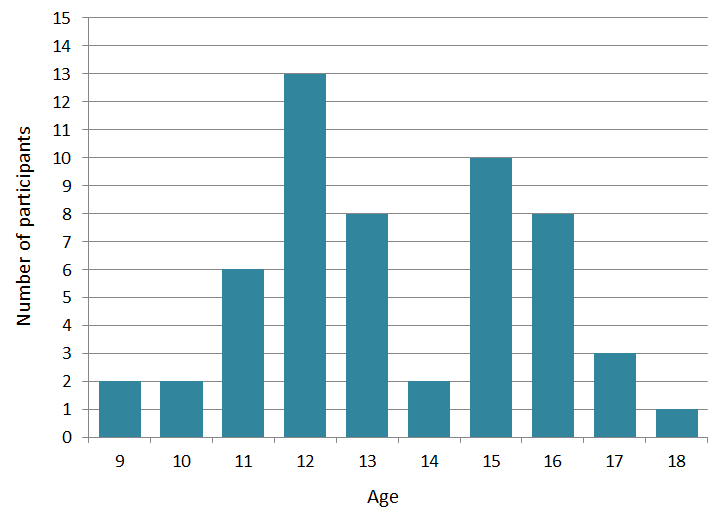
\includegraphics[width=0.5\columnwidth]{figures/Age.png}
  \caption{Histogram of the age of the participants in the survey.}
  \label{fig:age} 
\end{figure*}

An investigation among the boys and girls was performed to determine if there were any differences regarding their activities during the event.
Figure~\ref{fig:activities} shows the participation in the various activities in respect to gender. 
It was observed that there was a radical difference between male and female participants. 
For example, looking at the activity related to the programming of the robot, it was denoted that girls did not interact much with Thymio II during the event. 
%Also when analyzing what knowledge and experience children had at the end of the project, we denoted that only 73 percent of girls had the experience in programming of the robot, when it was 100 percent for the boys, meaning that the girls learned to program the robot from basics. 
Figure~\ref{fig:activities} also shows that the girls were clearly more devoted to tasks related to communication, which explains why they did not program the robots. 
This result shows that it could be interesting to oblige the children to try all the different tasks, which could compensate for this natural trend and provide a more balanced experience.

\begin{figure*}[ht]
 \centering
    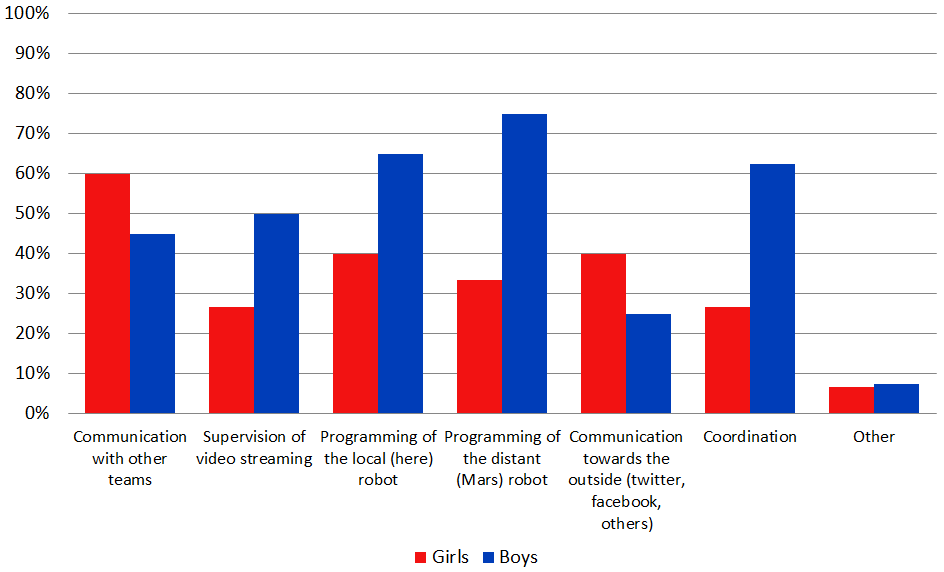
\includegraphics[width=0.7\columnwidth]{figures/activities.png}
  \caption{Activities performed during the event by girls and boys.}
  \label{fig:activities} 
\end{figure*}

Figure~\ref{fig:tele} shows the opinions of the participants regarding telerobotics. 
Initially, it can be seen that there was a lot of very positive appreciation. 
Even though the children felt that ``telerobotics requires more reflection on the program'' as well as before programming, at the same time they agreed that ``telerobotics brings more fun.'' 
They seemed to enjoy this challenging aspect of the project, which is very important from an educational perspective. 
In addition, nearly 90\% of the participants thought that this activity required teamwork, which obliged them to coordinate better within their teams. 
Finally, one can see that nearly 30\% of the children disagreed with the statement ``telerobotics is closer to a real use of robots'' or that ``a remote robot need to be programmed differently than a robot physically accessible near you.''
Both sentences, although they pull in opposite directions, imply a difference between telerobotics and other approaches.

Some of the children probably saw telerobotics at the same time closer to real problems than what they saw until then, and to be programmed differently than robots physically accessible.
One element worried us during the event: participants sometimes had to wait a long time for another group before being able to move forward with their mission. 
This was the reason for our question about how boring telerobotics is.
The result of the survey is encouraging, as less than 15\% found it boring.


\begin{figure*}[ht]
 \centering
    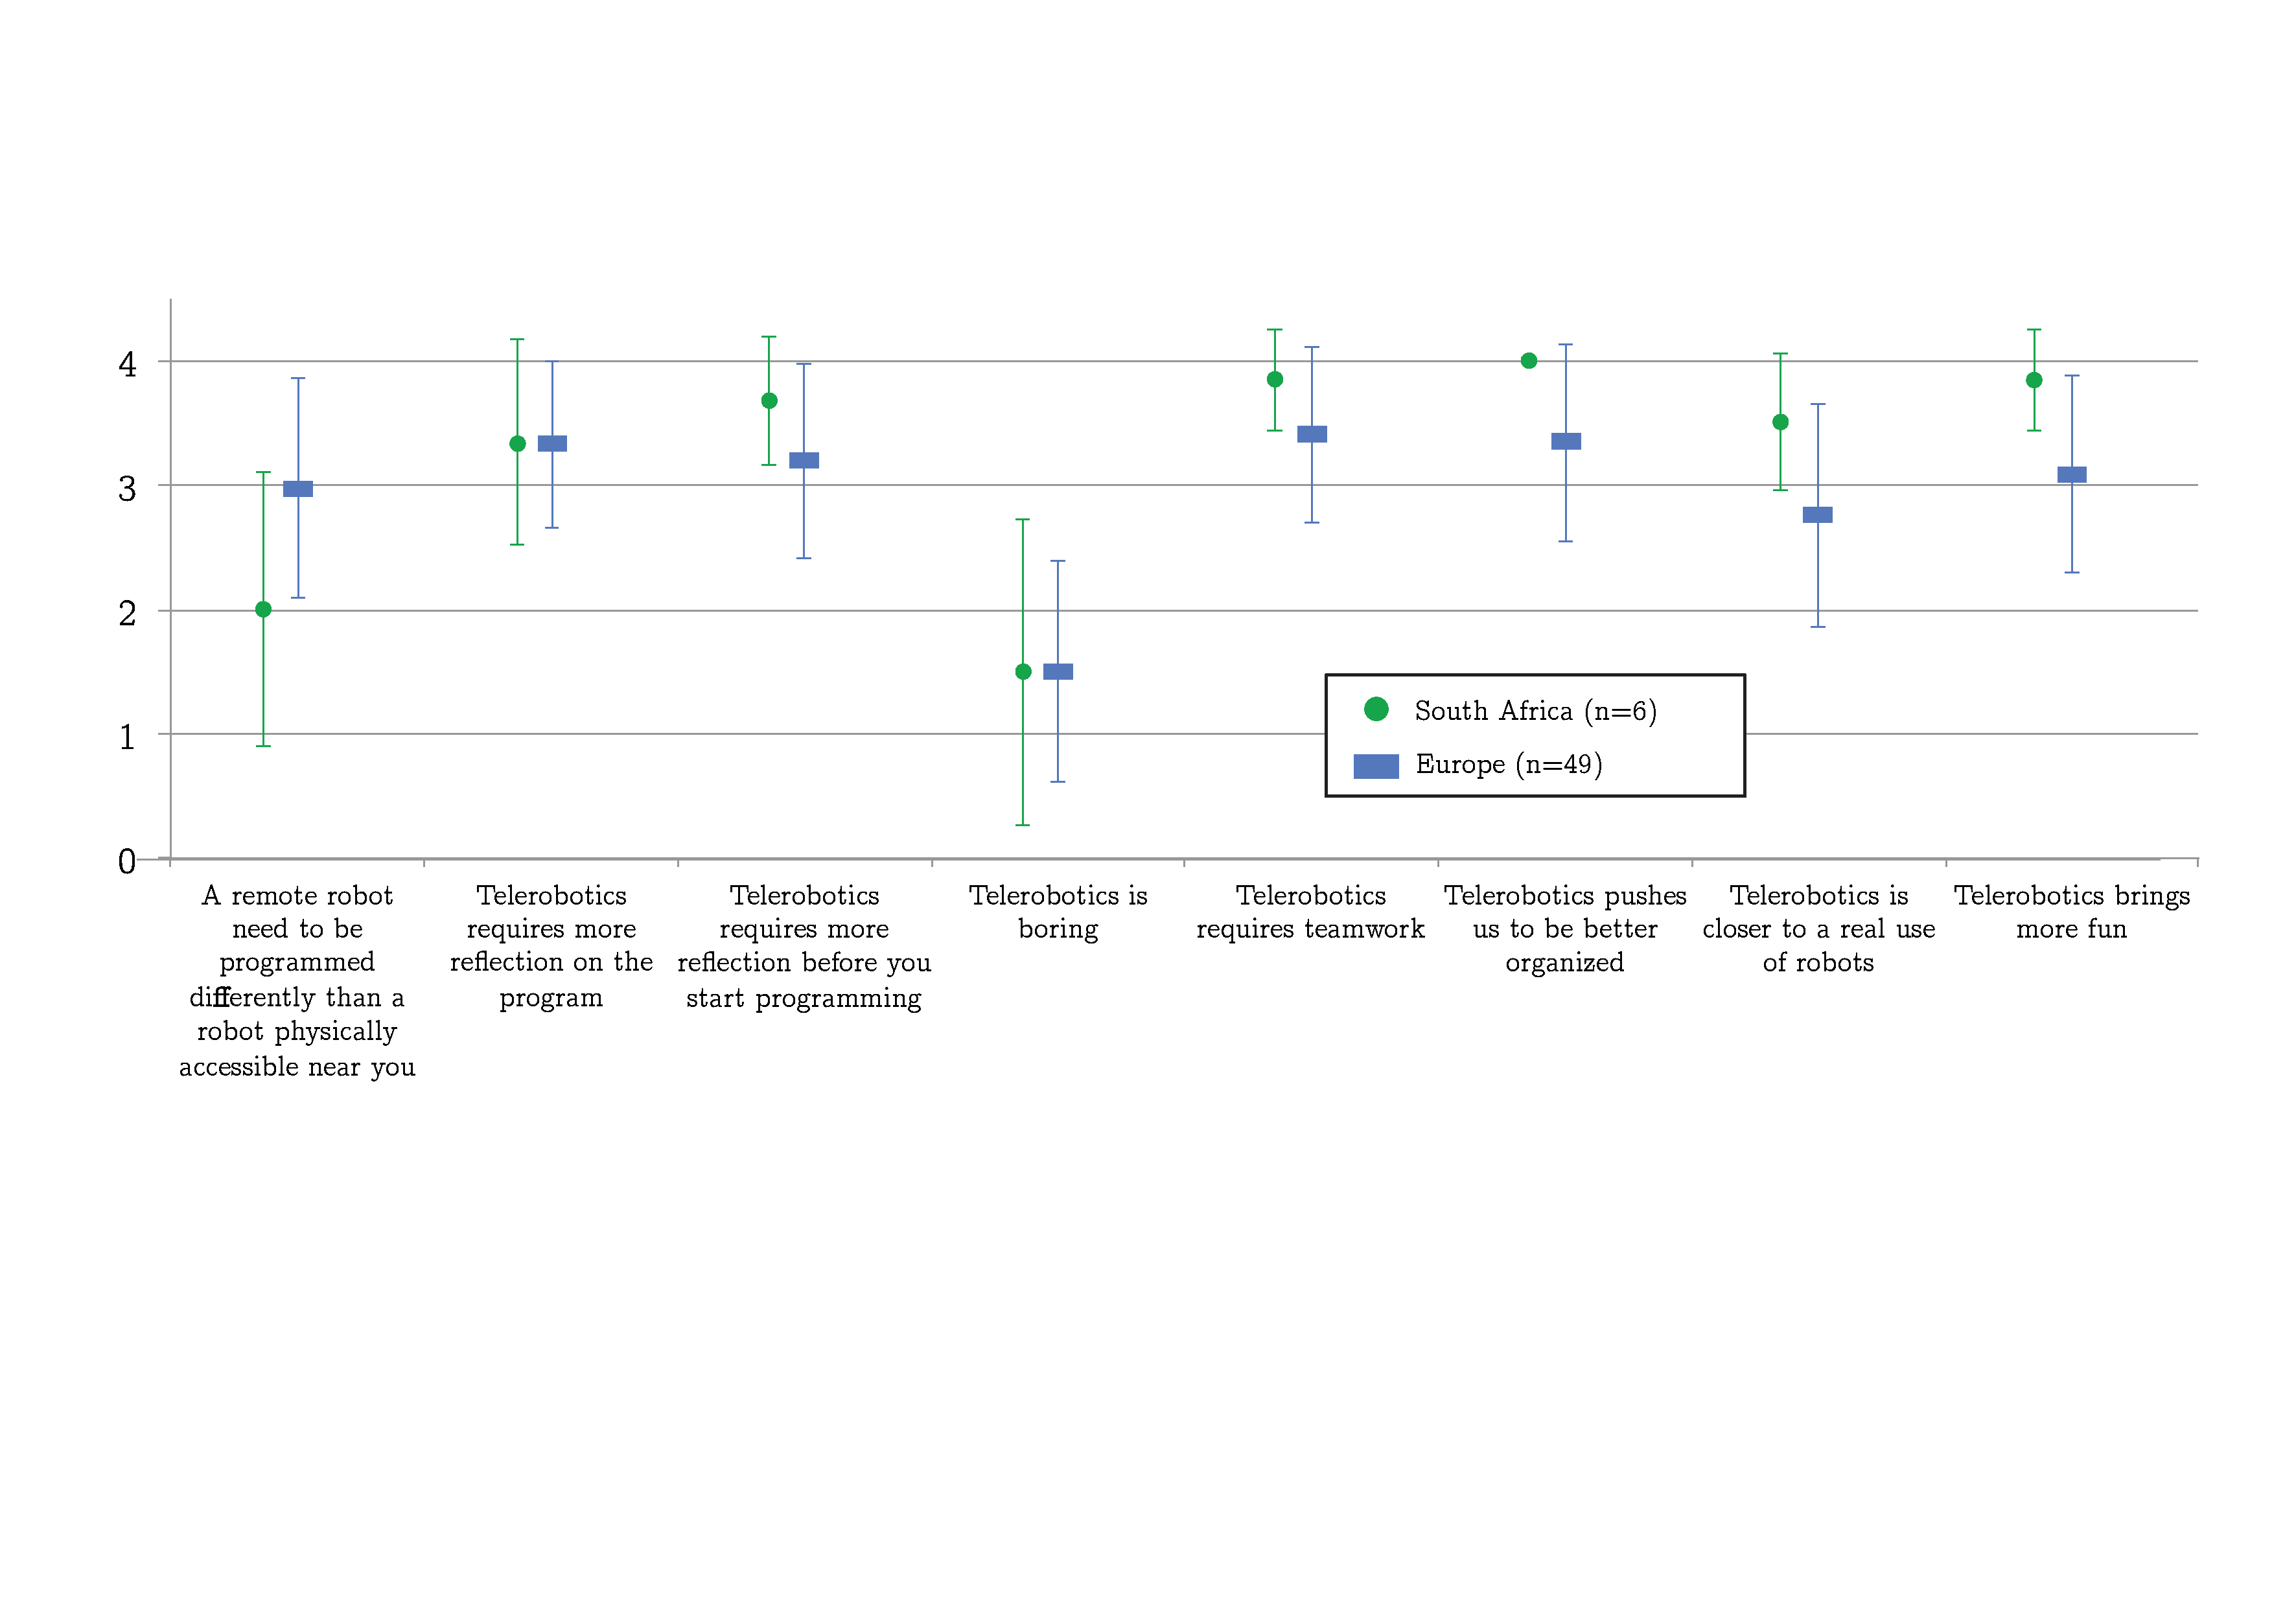
\includegraphics[width=\columnwidth]{figures/telerobotics.pdf}
  \caption{Feedback about telerobotics.}
  \label{fig:tele} 
\end{figure*}

The children were also asked whether they have learned about new topics by participating in R2T2 (Figure~\ref{fig:robotics}). 
The general level of appreciation was extremely high, with answers that were 70\% to 90\% positive for all points beginning with ``I learned.''
The highest score was for ``I learned to work in a team'', which is a key element of this event, especially if combined with the 94\% who stated that ``I had fun''; this shows that this learning process is enjoyable.
The lowest score among the learned skills was for ``I learned to program a robot'', as 71\% of the participants stated that they had programmed a robot before.
However, the special nature of the task meant that more than 80\% stated that ``I learned to program differently.''
The number of participants finding ``everything quite slow and boring'' was also low, with 65\% of totally disagreeing. 
This result is highly positive, as mentioned above, because the R2T2 event was quite long and there was a risk that the children would get bored waiting. 

\begin{figure*}[ht]
 \centering
    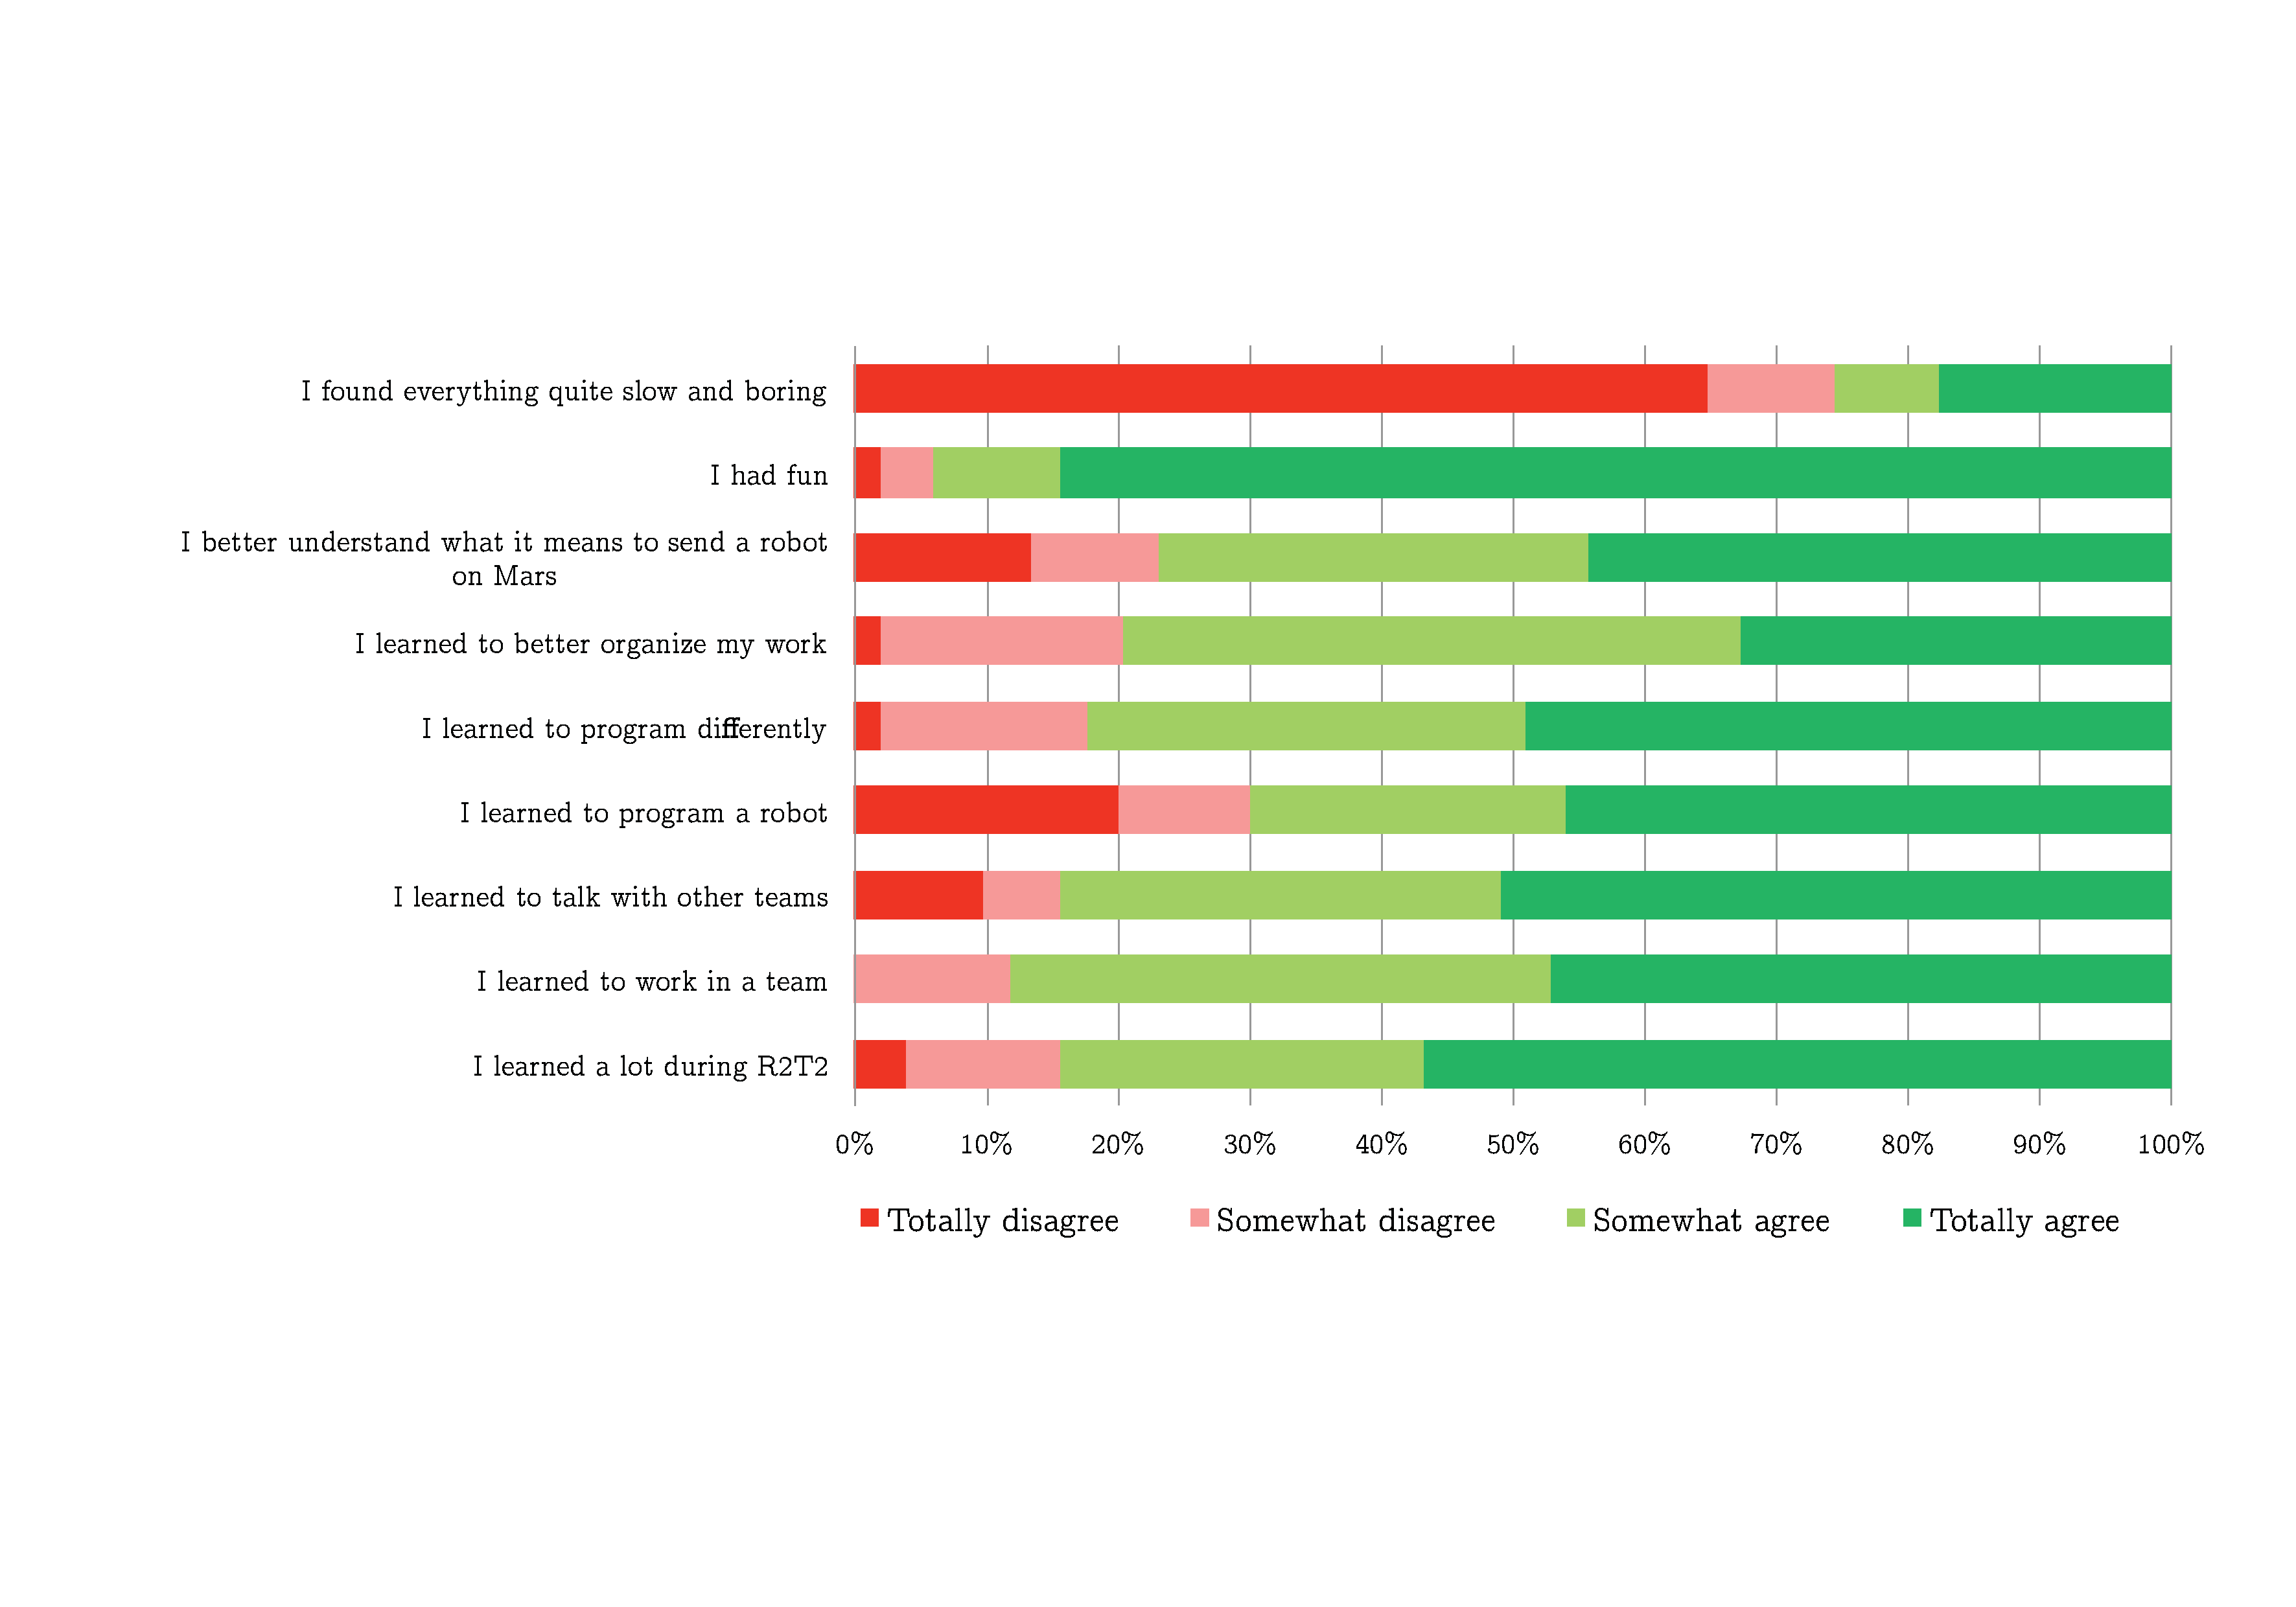
\includegraphics[width=0.9\columnwidth]{figures/robotics.pdf}
  \caption{Feedback about the robotics experience.}
  \label{fig:robotics} 
\end{figure*}

Figure~\ref{fig:learned} shows the superimposition of figures concerning competences available before the event and what the participants perceived that they had learned.
This confirms several other observations made above.
In particular, we have confirmation that female participants started with lower competences in robot programming, but also learned much less than their male colleagues. 
The situation is similar for another technical aspect of the activity, video streaming. 
Meanwhile, for communication, it is the opposite, the males considering that they had learned as much as the females. 
It is hard to determine whether the girls were limited in their choice or if they preferred this role because they were more competent in this area. 
What is clear is that this event attracted a higher number of female participants than traditional robotic events, which is already a positive element.
Another less positive observation is that the activity amplified the male-female gap, at least in terms of learning. 


\begin{figure*}[ht]
 \centering
    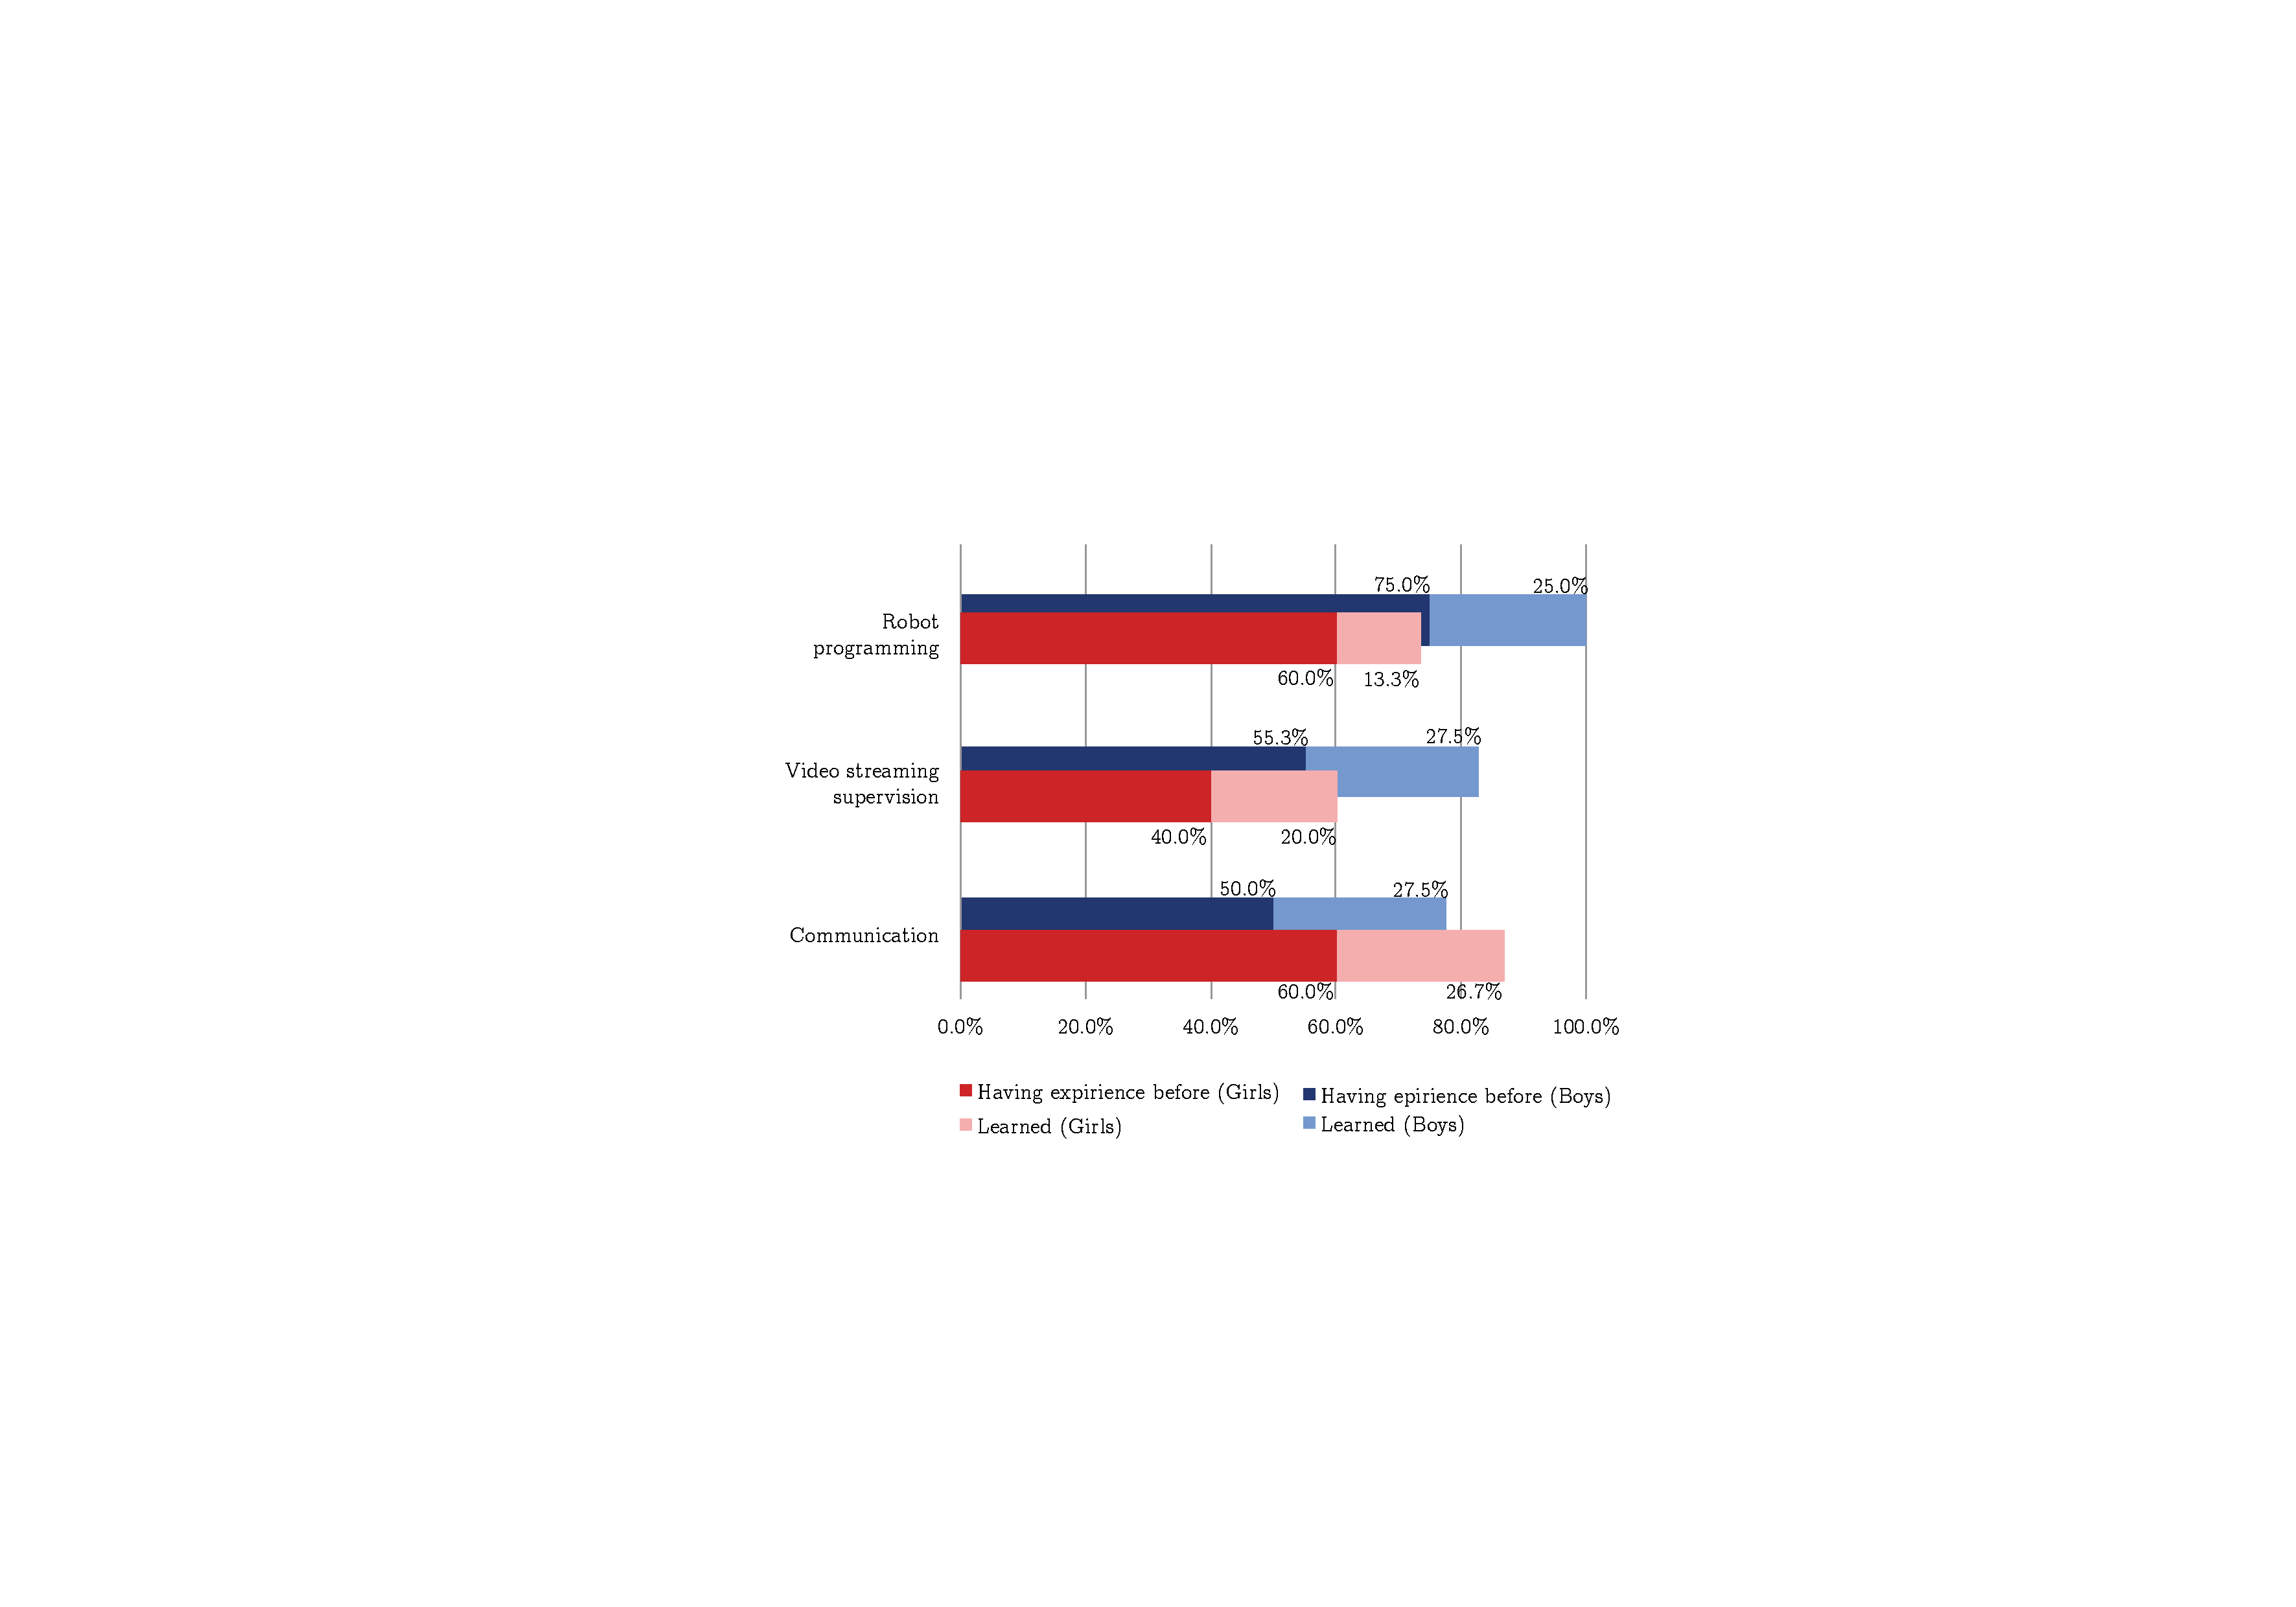
\includegraphics[width=0.6\columnwidth]{figures/learned.pdf}
  \caption{Combination between learned skills and previous competences.}
  \label{fig:learned} 
\end{figure*}

\subsection{Results of the survey: Africa versus Europe}

After having looked into the general impact of the activity, one can examine in more detail the answers of the European and African participants. 
Although the survey was anonymous, the IP number of the computer used to enter the survey was used to extract the country of the participants.
This analysis has to be considered with care, as only eight participants represented South Africa in this survey, against 49 for Europe.


Figure~\ref{fig:EU-SA} shows an overall picture on all feedback about telerobotics and learning.
What is readily apparent is that African participants tended to be more enthusiastic, had a higher consideration for the activity, and perceived that they had a higher learning outcome. 
For several statements, we had 100\% agreement from South African participants: ``I had fun'', ``I learned a lot in R2T2'', and ``Telerobotics pushes us to be better organized.''
Together, these three statements give a clear indication of the attitude towards this activity in South Africa; it perfectly mixes fun and learning, but also includes in the learning experience several methodological aspects that we had already observed during the preparation of the team. 

\begin{figure*}[ht]
 \centering
    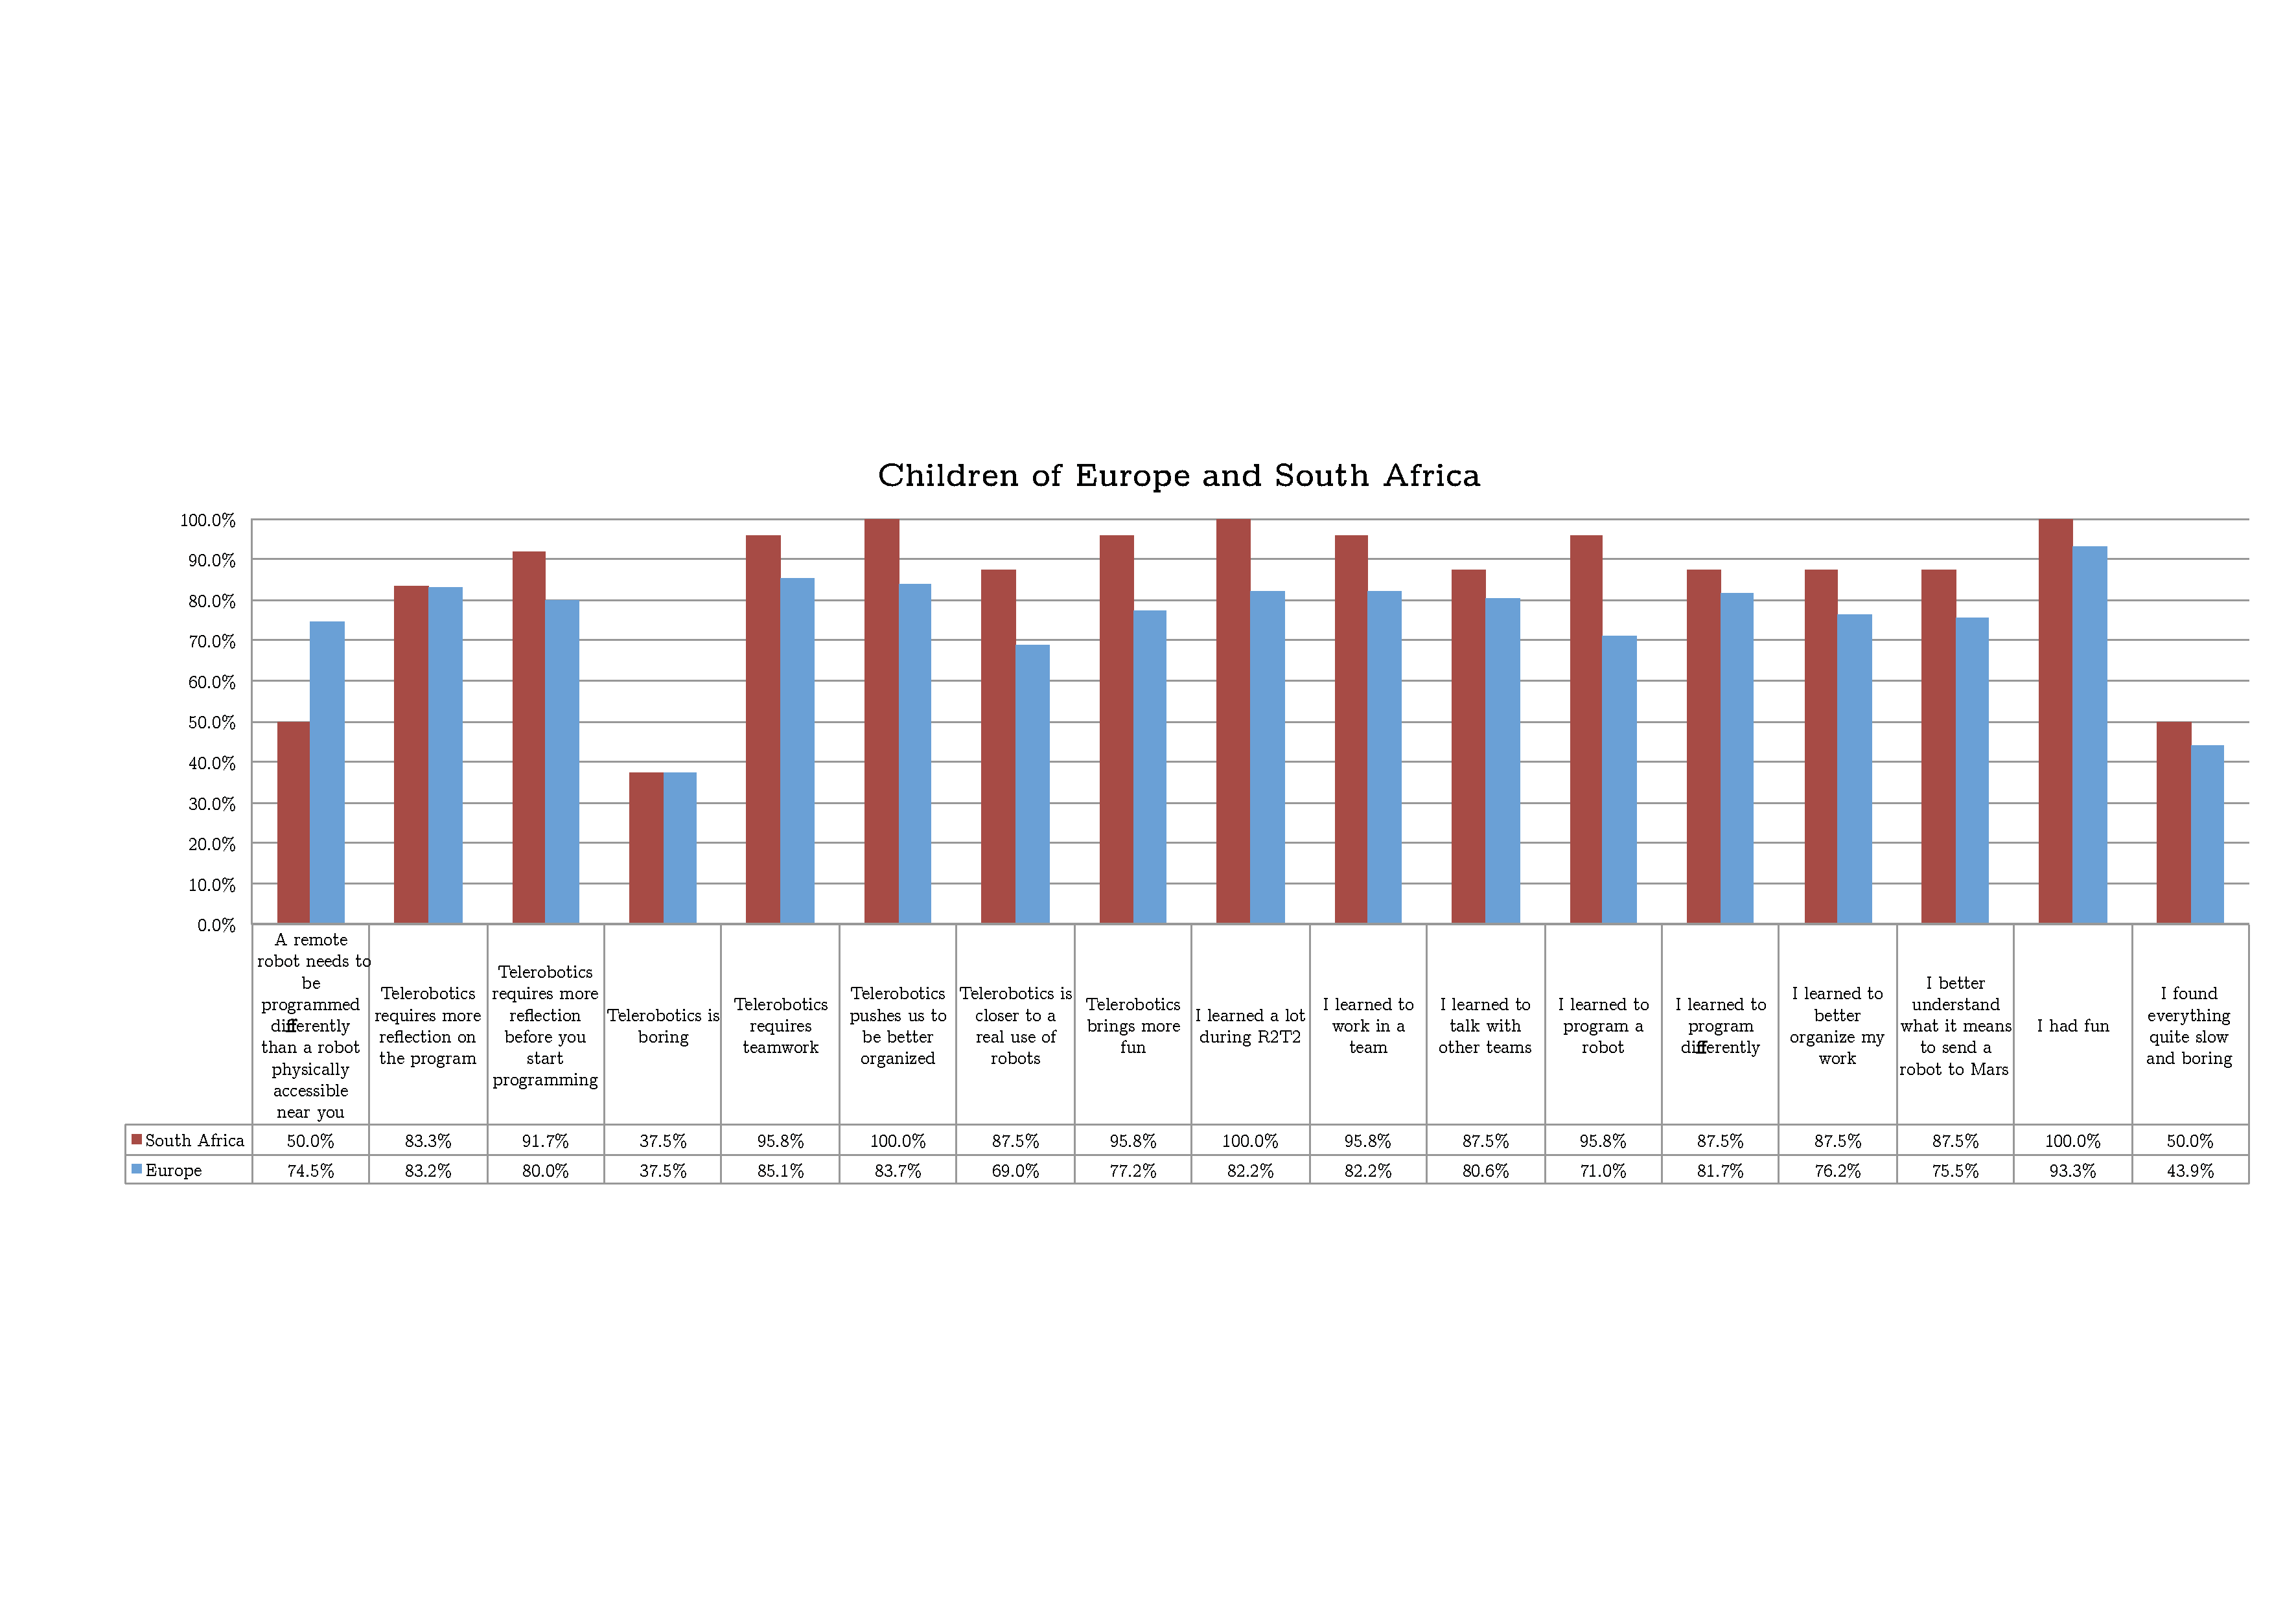
\includegraphics[width=\columnwidth]{figures/all-eu-sa.pdf}
  \caption{Comparison between survey responses by participants from Europe and Africa.}
  \label{fig:EU-SA} 
\end{figure*}

If one looks again at the added value of the activity, expressed as a comparison between competences that the participants had before the event and those they consider as having learned, the results illustrated in Figure~\ref{fig:EU-SA-learn} are obtained.
This shows a dramatic difference in competences before the event between African and European participants, with the African ones having very little experience in the technologies used in this activity, and the Europeans having very good experience, especially in robot programming. 
The perceived learning impact is much more important for African participants than European ones. 

\begin{figure*}[ht]
 \centering
    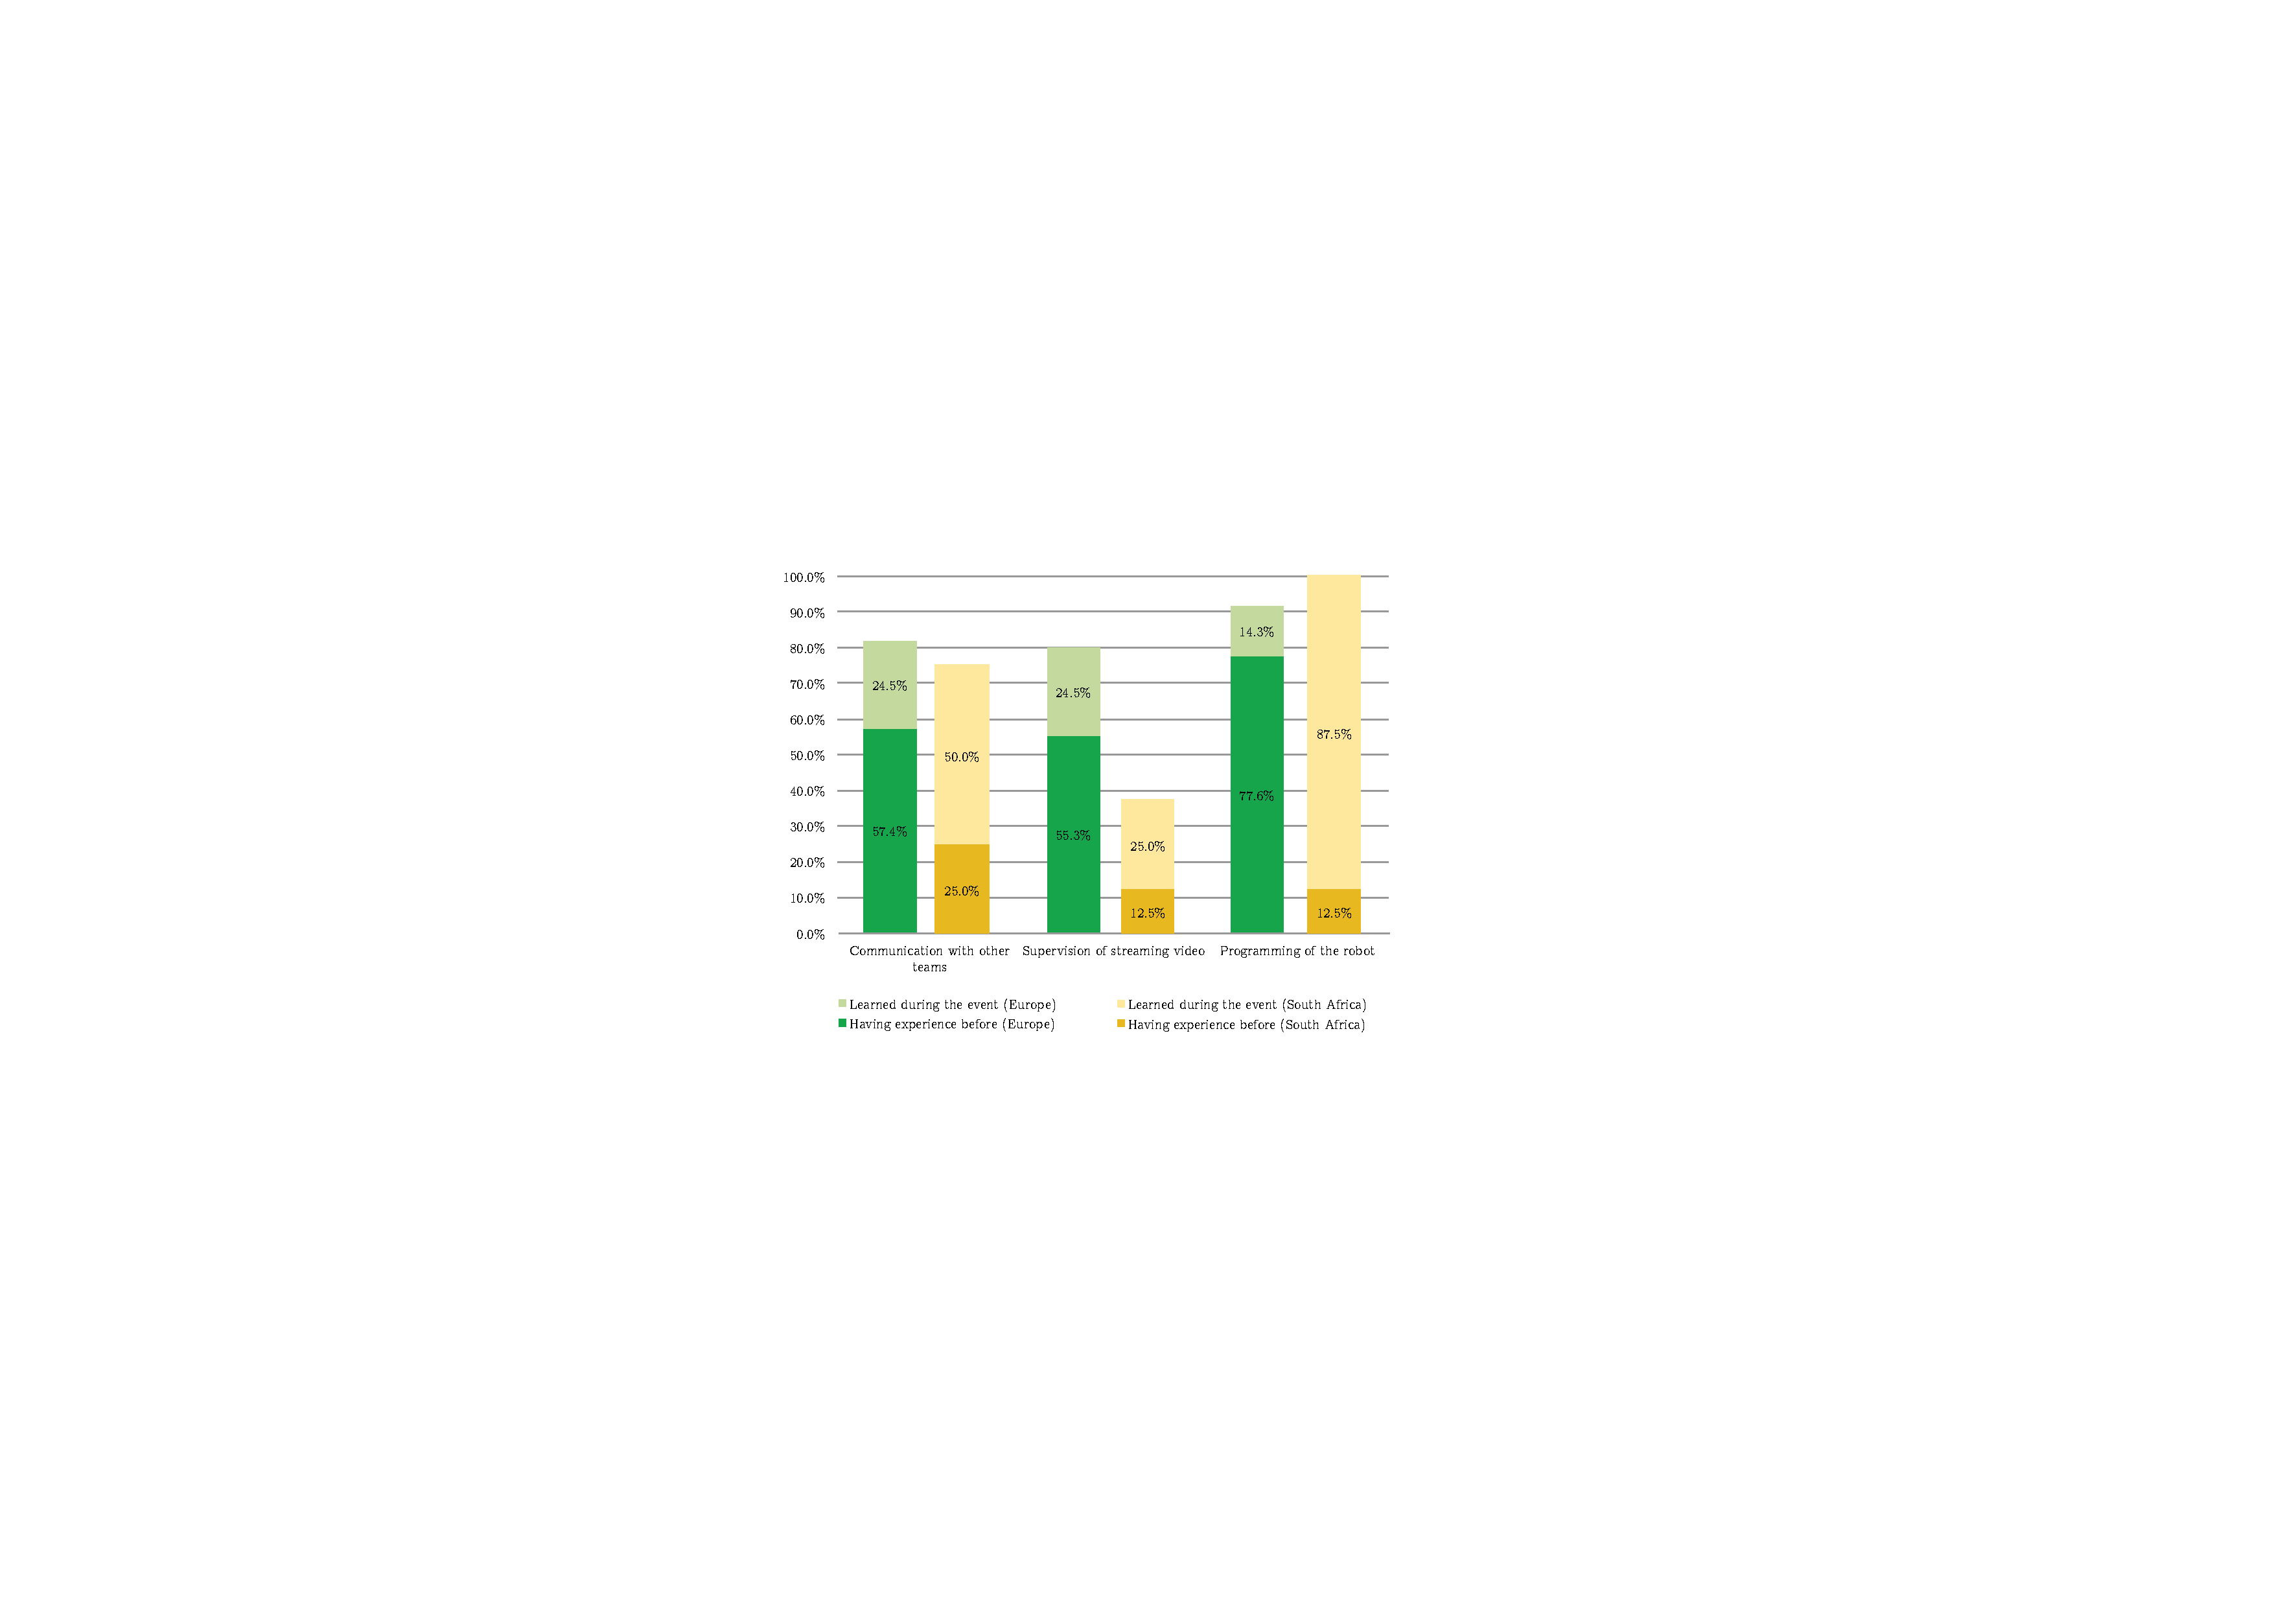
\includegraphics[width=0.6\columnwidth]{figures/EU-SA-learned.pdf}
  \caption{Comparison between survey responses by participants from Europe and Africa, looking at the combination between learned skills and previous competences.}
  \label{fig:EU-SA-learn} 
\end{figure*}


\section{Discussion and conclusion}

This first online integration of young students from Africa and Europe in a collaborative robotics activity has highlighted some difficulties of the approach, but also its impressive potential.

Among the problems, we can mention the language and the internet infrastructure.
The choice of French as a communication language, although common in several African countries, was problematic for South Africa.
Government schools in South Africa do not readily offer French as a language course.
Therefore, it was decided to select a secondary school that took into account the requirement of having at least one team member who was fluent in French. 
The other problem was the Internet, due to the limited bandwidth. 
The two YouTube video streams used as video feedback were very choppy and the sound was not streamed properly.
It was also observed that when viewing the same video stream through a smartphone and a GPRS signal, a different video footage was observed. 
This was challenging for the participants, creating a kind of insecurity when sending a robot command.
It was planned to stream back the video of the team, but finally it proved to be unfeasible, as the YouTube footage was not recorded properly.

Despite these problems, the potential of the concept has been shown to be impressive.
In general, all participants were enthusiastic about the topic, the challenge, the international nature of the event, and the broad spectrum of activities. 
Some of the coaches, who could qualitatively compare the engagement of the participants in this event with that seen in robot competitions, assessed it as being very similar, despite the collaborative nature of the task. 
However, in contrast to robot competitions, none of the teams had to accept a defeat at the end of the day, as all were equally successful. 
In South Africa in particular, the theme of the event attracted the top students from various grades within the selected school. 
These students formed the team that participated in the event; all of them had prior experience with programming hobby kits such as the Arduino Uno programmable controller. 
The initial team of four members rapidly expanded to twelve, and the original team took it upon themselves to train their peers who showed interest. 
The training of the team was made easier by the fact that the selected students had prior programming knowledge. 
A set of instructions was supplied with the Thymio kit, along with a training manual which introduced the user to the various functions and capabilities of the robot. 
The method used to train the students involved implementation of the training manual, which was supplemented by the allocation of tasks specific to the environment in which the team worked. 

The delay introduced by the video streaming, and the impossibility of physically accessing the robots, radically changed the way in which the participants could approach the problem.
Rapid coding and testing without thinking became impossible, as the download and execution of code in the robot had a high cost in time and the results could not be reversed. 
In addition, the effect could be observed only after an important delay, increasing the impact of mistakes.
This way of working, which was complex and closer to a real engineering situation, was highly appreciated by the participants, who had a hard time solving the task but, at the same time, clearly had fun during the afternoon.
In particular, they were challenged on their coordination, preparation, thinking before programming, and so on. 
A great majority of the participants reported having learned a lot about team coordination and methodology of work, which is a key element in learning.
In South Africa, in particular, the participants thought that they could give the Thymio robot instructions and get things working the first time, even though they were advised not to do so. 
The participants were frustrated at times when things did not happen as they expected, but once they realized that they had to solve the problems using smaller steps and in a sequential manner, they had more success. 
They learned very quickly to follow the advice and to work in a team, first to simulate instruction on the robot they had within the lab, before sending the instruction to the robot.
After the participants changed their approach, they rapidly became more successful in attempting the challenges. 

The most challenging aspect of the teaching of robotic systems in South Africa is the methodology, with the sequential steps in the programming of the robots. 
It is found that the scholars are able to grasp the mechanical component quite easily, as they have been exposed to building structures, whether it is with sand, stones, sticks, or even more advanced material such as building bricks, Lego blocks, or metal materials. 
Understanding the electronic component is a little more difficult, yet as the students are exposed to more electronic systems and are taught electrical circuits from a young age, they are able to connect the different components and modules. 
The aspect that scholars have difficulty with is the programming. 
Even though the R2T2 participants were taught to plan with flowcharts and pseudocode, and informed that they must think of themselves as the robot in terms of the steps that needed to be followed, the students had difficulty with methodic approach. 
The R2T2 activity is an extremely elegant way to bring them to a situation where they can well understand by their practice how important it is to address problems with a clear methodology. 
Their feedback in the survey shows that they grasped the importance of this aspect and learned how to improve it.

%There are many factors for the scholars to have a difficulty to understand this concept, and it could be due to everything happening lately automatically, with less problem solving, as technology has developed, and also due to scholars not being exposed to programming at a younger age. Typically, within South Africa, some scholars are only exposed to programming for the first time in grade 8, otherwise only in grade 10 should they have taken computer science as a secondary school subject. It has also been found that some students are only exposed to programming when they reach university level, as their school did not have computer facilities and limited technology equipment. It is believed that this hurdle will only be overcome once programming skills are to be taught from the beginning of the scholar's school career, which can be pursued with activities such as placing the sequence of event into order with the different activities they need to perform to get to school every morning. Similar activities will make the scholars to have a better understanding with sequential programming in the future.

This very broad nature of the activity, including communication, strategy, planning, coordination, understanding and programming, has also shown several extremely interesting side effects.
The first, highlighted by the results of the survey, is a particularly high participation and specific role of female participants.
For example, it is hard to say if their strong participation in the communication roles is an interesting motivation factor or a limiting factor in respect to programming. 
What is much clearer is that the broad spectrum of disciplines included in R2T2 created a situation where several coaches were not computer scientists. 
It was seen among the teachers that French professors were interested in the experience of communication, or physics professors were interested by the space aspect of the event. 
It cannot be proven, but one can speculate that this also helped in getting a broader spectrum of participants, breaking the pattern of attracting only STEM-interested people.

Finally, the perception of learned lessons by the participants is impressive, especially among the participants of South Africa.
Their inclusion in an activity involving European participants, who have a better background in technological fields, can have a clearly positive impact through emulation, instead of competition as often practiced. 

\section{Future Work}
The learning quality of engineering disciplines has to face several issues in developed countries, such as distance and cost of materials, which could be addressed through distance learning~\cite{winthrop2012new}. 
This first R2T2 event showed how distant participation in a common event can not only impact costs of infrastructure and travel, but can bring key educational elements and promote inclusion at various levels, not only among geographically far countries, but also among disciplines and genders.

Strong from this first R2T2 experience, we plan to use the platform for more events in order to connect people between Southern and Northern countries (or between companies and engineering schools for example). 
We noticed that communication and collaboration was a valuable skill for this learning task.
Hence, the fact that participants spoke the same language was crucial and enriched the event with a cultural exchange aspect.
In the future, we plan to stimulate this exchange medium by proposing events to connect other francophone countries around the world. 

We also plan to make the R2T2 environment more attractive by adding embedded cameras on the robots making tele-operation more immersive. 
With time, we expect to build an international network of schools and participants who would regularly use the R2T2 platform. 
\small
\bibliography{r2t2}{}

\end{document}